%&../../.preamble
\externalize{../../.preamble}

\usetikzlibrary{patterns}
\usetikzlibrary{decorations}
\usepackage{multirow}
\usetikzlibrary{angles, quotes, calc}


\title{Ripetizioni Emma}
\author{Marini Mattia}
\date{2023 2024 2025}

\begin{document}
\maketitle

\license{Dispense di matematica e fisica}

\tableofcontents
\newpage
\listoftables
\listofdefs
\listoftheorems
\listofexercises


%\section{Polinomi}
%\esercizio{Semplifica i seguenti polinomi}{
%  \begin{align}
%    & \left(a^2  - \frac{1}{3} ab\right) \left(\frac{1}{3} ab + a^2 \right)- \left(\frac{1}{3}a ^3 - ab\right)^2  + \frac{1}{9}a^2 \left(10b^2 +a^2 \right)\\
%    & \frac{\left[\left(x^n-y^n\right)\left(-x^n-y^n\right)- \left(x^n + y^n\right)^2 \right]x^n -2\left(-x^n \right)^{3}}{\frac{-1}{2}x^{2n}}
%  \end{align}
%  }
%  \subsubsection{Soluzioni}
%  \begin{enumerate}
%    \item 
%      \begin{align*}
%        & \underbracket[0.1ex]{\left(a^2  - \frac{1}{3} ab\right) \left(\frac{1}{3} ab + a^2 \right)}_{\text{ somma per diff }}- \underbracket[0.1ex]{\left(\frac{1}{3}a ^3 - ab\right)^2}_{\text{ quadrato bin }}  + \frac{1}{9}a^2 \left(10b^2 +a^2 \right)\\[10pt]
%        &= a^{4} + \frac{1}{9}a^2  b^2 \frac{-1}{9}a^{6}-a^2 b^2    + \frac{2}{3}a^{4}b   + \frac{10}{9}a^2  b^2  + \frac{1}{9}a^{4}\\[10pt]
%        &= \frac{10}{9}a^{4} - \frac{1}{9}a^{6}+ \frac{2}{3}a^{4}b\\[10pt] 
%      \end{align*}
%\item \begin{align*}
%    & \frac{\left[\left(x^n-y^n\right)\left(-x^n-y^n\right)- \overbracket[0.1ex]{\left(x^n + y^n\right)^2}^{\text{ quadrato bin }} \right]x^n -2\left(-x^n \right)^{3}}{\frac{-1}{2}x^{2n}}\\
%    & \frac{\left[\overbracket[0.1ex]{\left(x^n-y^n\right)\left(x^n+y^n\right)}^{\text{ somma per diff }}\left(-1\right)-x^{2n} - y^{2n} - 2x^{n}y^{n} \right]x^n -2x^{3n}}{\frac{-1}{2}x^{2n}}\\
%    & \left\{\left[-x^{2n} + y ^{2n} - x^{2n} - y^{2n} - 2x^{n}y^{n}\right]x^{n}\right\} \left(\frac{-2}{x^{2n}}\right)\\ 
%    & \left\{\left[-2n^{2n} - 2n^{n}y^{n}\right]x^{n}\right\}\left(\frac{-2}{x^{2n}}\right) \\
%    & \left(- 2x^{3n} - 2x^{2n}y^{n} + 2x^{3n}\right) \left(\frac{-2}{x^{2n}}\right)\\
%    &4y^{n}
%\end{align*}
%  \end{enumerate}
\newpage
\section{Prodotti notevoli}

\subsection{Proprietà potenze}
\begin{align*}
	a^{n}a^{m}             & = a^{n-m}        \\[12pt]
	a^{-1}                 & = \frac{1}{a}    \\[12pt]
	\left(a^{n}\right)^{m} & = a^{n \cdot  m} \\[12pt]
\end{align*}
\subsection{Prodotti notevoli}\label{prodnotevoli}
\begin{align*}
	\left(a + b\right)^2 & = a^2  + b ^2  +2ab                           \\[12pt]
	\left(a + b\right)^3 & = a^3  + b^3 +3a^2 b + 3 a b^2                \\[12pt]
	a^2  - b^2           & = \left(a+b\right)\left(a-b\right)            \\[12pt]
	a^3 + b^3            & = \left(a + b\right)\left(a^2 +b^2 -ab\right) \\[12pt]
	\left(a+b+c\right)^2 & = a^2  + b^2  + c^2 +2ab + 2ac + 2bc
\end{align*}
\subsection{Domande interrogazione}
\begin{enumerate}
	\item Qual è l'utilizzo dei prodotti notevoli? E' indispensabile il loro utilizzo?
	\item Dimostra come vengono derivate le formule dei prodotti notevoli enunciate in sezione \ref{prodnotevoli}
	\item Dimostra come sia possibile passare dalla formula con il più alla formula con il meno in questi casi
	      \begin{align*}
		      \left(a+b\right)^2 = a^2  + b^2 + 2ab                      & \rightarrow \left(a-b\right)^2 =a^2  + b^2 - 2ab                      \\
		      \left(a + b\right)^3 = a^3  + b^3 +3a^2 b + 3 a b^2        & \rightarrow \left(a - b\right)^3 = a^3  - b^3 -3a^2 b + 3 a b^2       \\
		      a^3  + b^3 = \left(a+b\right)\left(a^2  + b^2  - ab\right) & \rightarrow a^3  - b^3 =  \left(a-b\right)\left(a^2  + b^2 +ab\right)
	      \end{align*}
	      Come mai non esiste un prodotto notevole per la forma $ a^2  + b^2  $? Come mai non possiamo ricavare il prodotto notevole per questa forma partendo dalla forma con il meno $ a^2  - b^2  $?
\end{enumerate}

\section{Equazioni fratte}
Nel momento in cui dobbiamo risolvere delle equazioni fratte è fondamentale avere delle tecniche per semplificare l'espressione. Per semplificare l'espressione bisogna riuscire a scrivere i polinomi come \underline{prodotto polinomi di grado inferiore}:
\[
	\frac{x^2 -x - 2}{x+1} = \frac{\left(x-2\right)\left(x+1\right)}{x+1}
\]
in questo caso, il membro a destra risulta molto più comodo di quello a sinistra in quanto è scritto come prodotto di polinomi, i quali possono essere semplificati:
\[
	\frac{\left(x-2\right)\left(x+1\right)}{x+1} = x-2
\]
lo scopo delle prossime pagine sarà quello di trovare tecniche per \underline{scomporre i polinomi}, permettendo quindi di semplificare le fratte
\subsection{Raccoglimento totale}
Questo metodo si basa sulla proprietà distributiva "applicata al contrario":
\[
	A \cdot B + A \cdot C = A\left(B + C\right)
\]
Lo stesso ragionamento può essere fatto con i polinomi:
\[
	2x a + 2x b = 2x \left(a + b\right)
\]
oppure
\[
	4x^3  + 2x^2  = 2x^2  \cdot 2x + 2x^2  = 2x^2  \left(2x +1\right)
\]
\begin{tcolorbox}
	Idea del raccoglimento totale:
	\begin{itemize}
		\item Cerco il fattore comune (ossia il monomio che divide tutti gli altri) che abbia esponente maggiore
		\item Moltiplico il fattor comune per gli tutti i membri divisi a loro volta per il fattor comune stesso
	\end{itemize}
\end{tcolorbox}

\subsection{Raccoglimento parziale}
Quando un polinomio è composto dalla somma di 4 monomi si può applicare il raccoglimento totale a due a due, per poi raccogliere ancora una volta:
\[
	\underbracket[0.1ex]{3ax + 3bx}_{\text{ raccolgo }} + \underbracket[0.1ex]{ay + by}_{\text{ raccolgo }} = \underbracket[0.1ex]{3x\left(a + b\right) + y\left(a + b\right)}_{\text{ raccolgo }} = \left(a+b\right)\left(3x + y\right)
\]
La sfida qui sta nel cercare la combinazione che mi permetta di raccogliere una seconda volta. Un consiglio può essere quello di \underline{raccogliere i membri il cui rapporto fra i coefficienti sia lo stesso}

\subsection{Trinomio speciale}
Quando abbiamo un polinomio di secondo grado, possiamo a volte scomporlo tramite questo "algoritmo". Dato $ P\left(x\right) $
\[
	ax^2 +bx + c
\]
\begin{itemize}
	\item Cerco due numeri interi $ x_1 $ e $ x_2 $ che sommati diano $ b $ e moltiplicati $ a \cdot c $
	\item In questo caso $ a $ e $ b $ esistono e sono 2 e -3
	\item Se $ a=0 $ allora posso riescrivere il polinomio direttamente come
	      \[
		      \left(x + x_1\right)\left(x + x_2\right)
	      \]
	\item Altrimenti rischiviamo il polinomio rimpiazzando il il termine di primo grado con $ \left(x_1 + x_2\right)x $ ed effettuiamo raccoglimento parziale, il quale è garantito che riesca
\end{itemize}
Ad esempio con
\[
	x^2  -x -6
\]
i due numeri candidati sono 2 e -3: Allora possiamo riscrivere il polinomio come:
\[
	\left(x+2\right) \left(x-3\right)
\]
\subsection{Formula risolutiva eq secondo grado}
Se non si riesce a scomporre un polinomio con il metodo appena enunciato, è possibile utilizzare la seguente formula. Dato un polinomio $ ax^2  + bx + c $, troviamo gli zeri:
\[
	x_{1 / 2} = \frac{-b \pm \sqrt{b^2 - 4ac}}{2a}
\]
otteniamo quindi due numeri $ x_1 $ e $ x_2 $(uno utilizzando il + e uno utilizzando il - nella formula sopra). Scriviamo ora il polinomio come
\[
	a\cdot \left(x-x_1\right)\left(x-x_2\right)
\]

\subsection{Prodotti notevoli}
Utilizzando "al contrario" i prodotti notevoli elencati in sezione \ref{prodnotevoli}, possiamo scrivere un polinomio come prodotto
\section{Disequazioni}
La differenza nella risoluzione di un'equazione e di una disequazione sta principalmente nell'ultimo step e nel fatto che bisogna stare attenti a dividere/moltiplicare per quantità negative.

\subsection{Disequazioni letterali di primo grado}
Voglio arrivare ad una forma di questo tipo:
\[
	Ax < B
\]
Il metodo generale per risolvere una disequazione \underline{non fratta} è il seguente:
\begin{itemize}
	\item Svolgo calcoli a destra e a sinistra del $ < $ o $ > $
	\item Porto alla sinistra tutto ciò che contenga l'incognita (es $ 2x, ax, ab\left(x\right) $) e a destra tutto ciò che non la contiene (es $ 13, a, ab $)
	\item Raccolgo la $ x $ a sinistra e studio il parametro se presente. Avrò una forma di questo tipo:
	      \[
		      Ax < B
	      \]
	      Al posto di $ < $ chiaramente ci possono essere $ > \le \ge  $
	      \begin{itemize}
		      \item Verifico cosa succede quando $ A = 0 $
		      \item Verifico cosa succede quando $ A>0 $ La soluzione è $ x < \frac{B}{A}  $
		      \item Verifico cosa succede quando $ A<0 $. La soluzione è $ x > \frac{B}{A}  $, ossia inverto l'uguaglianza
	      \end{itemize}
\end{itemize}
Per studiare il segno di $ A $ è necessario spesso usare le tabelle
\subsection{Disequazioni letterali fratte}
Voglio arrivare ad una forma di questo tipo:
\[
	\frac{A}{B} < 0
\]
dove $ A $ e $ B $ sono polinomi
\begin{itemize}
	\item Svolgo i calcoli e porto tutto a sinistra
	\item Studio il segno del numeratore
	\item Studio il segno del denominatore
	\item Nell'uso delle tabelle per lo studio del segno studio anche il segno del parametro
\end{itemize}

L'ultimo punto è la cosa che crea più confusione. Supponiamo di avere
\[
	\frac{x - 2a}{x - a} > 0
\]
Verrebbe automatico studiare il segno come segue:
\begin{center}
	\begin{tikzpicture}[xscale = 2]
		\draw (0,0)--(3,0);
		\draw (0,-1)--(3,-1);
		\path (0,0)--(1,0) node [midway, below]{-}
		--(2,0) node [midway, below]{-}
		--(3,0) node [midway, below]{+} ;
		\path (0,-1)--(1,-1) node [midway, below]{-}
		--(2,-1) node [midway, below]{+}
		--(3,-1) node [midway, below]{+} ;
		\draw (0,-2)--(3,-2);
		\path (0,-2)--(1,-2) node [midway, below]{+}
		--(2,-2) node [midway, below]{-}
		--(3,-2) node [midway, below]{+} ;
		\draw [dotted] (1,0)--(1,-2);
		\draw [dotted] (2,0)--(2,-2);
		%
		\node [fill = white, anchor = east] at (0,0) {$ N $};
		\node [fill = white, anchor = east] at (0,-1) {$ D $};
		\node [fill = white, anchor = south] at (2,0) {$ 2a $};
		\node [fill = white, anchor = south] at (1,-1) {$ a $};
		\node [blackdot] at (2,0){};
		\node [blackdot] at (1,-1){};
	\end{tikzpicture}
\end{center}

tuttavia chi ci dice che $ a $ vada "a sinistra" di $ 2a $? Questo infatti non è necessariamente vero, infatti se $ a<0 $ allora $ 2a<a $. Per questo dobbiamo contemplare entrambe le opzioni:
\begin{center}
	\begin{tikzpicture}[xscale = 2]
		\draw (0,0)--(3,0);
		\draw (0,-1)--(3,-1);
		\path (0,0)--(1,0) node [midway, below]{-}
		--(2,0) node [midway, below]{-}
		--(3,0) node [midway, below]{+} ;
		\path (0,-1)--(1,-1) node [midway, below]{-}
		--(2,-1) node [midway, below]{+}
		--(3,-1) node [midway, below]{+} ;
		\draw (0,-2)--(3,-2);
		\path (0,-2)--(1,-2) node [midway, below]{+}
		--(2,-2) node [midway, below]{-}
		--(3,-2) node [midway, below]{+} ;
		\draw [dotted] (1,0)--(1,-2);
		\draw [dotted] (2,0)--(2,-2);
		%
		\node [fill = white, anchor = east] at (0,0) {$ N $};
		\node [fill = white, anchor = east] at (0,-1) {$ D $};
		\node [fill = white, anchor = south] at (2,0) {$ 2a $};
		\node [fill = white, anchor = south] at (1,-1) {$ a $};
		\node [blackdot] at (2,0){};
		\node [blackdot] at (1,-1){};
		\node [draw, anchor = west] at (4, -1) {Se $ a>0 $};
	\end{tikzpicture}
	\begin{tikzpicture}[xscale = 2]
		\draw (0,0)--(3,0);
		\draw (0,-1)--(3,-1);
		\path (0,0)--(1,0) node [midway, below]{-}
		--(2,0) node [midway, below]{-}
		--(3,0) node [midway, below]{+} ;
		\path (0,-1)--(1,-1) node [midway, below]{-}
		--(2,-1) node [midway, below]{+}
		--(3,-1) node [midway, below]{+} ;
		\draw (0,-2)--(3,-2);
		\path (0,-2)--(1,-2) node [midway, below]{+}
		--(2,-2) node [midway, below]{-}
		--(3,-2) node [midway, below]{+} ;
		\draw [dotted] (1,0)--(1,-2);
		\draw [dotted] (2,0)--(2,-2);
		%
		\node [fill = white, anchor = east] at (0,0) {$ N $};
		\node [fill = white, anchor = east] at (0,-1) {$ D $};
		\node [fill = white, anchor = south] at (2,-1) {$ a $};
		\node [fill = white, anchor = south] at (1,0) {$ 2a $};
		\node [blackdot] at (1,0){};
		\node [blackdot] at (2,-1){};
		\node [draw, anchor = west] at (4, -1) {Se $ a<0 $};
	\end{tikzpicture}
\end{center}

\section{Grandezze fisiche e unità di misura}
\begin{definizione}{Grandezze fisiche}
	Le \underline{grandezze fisiche} sono le prorprietà di un oggetto o di un fenomeno che si possono misurare
\end{definizione}
Occhio che non tutte le caratteristiche di un oggetto sono grandezze fisiche, in quanto alcune non possono essere misurate (es. \underline{bellezza, originalità})
\vskip3mm
\begin{definizione}{Unità di misura}
	\underline{L'unità di misura} di una grandezza fisica è un campione, scelto di comune accordo in modo che sia riproducibile e invariabile con cui di confrontano tutte le grandezze di quel tipo
\end{definizione}
Il confrondo si effettua dicendo quante volte l'unità di misura è contenuta in un'altra. (matematicamente si effettua un rapporto). Nota che potrei anche dire che un tavolo è lungo \textit{"3 spanne"}, però questo sarebbe impreciso perchè non tutte le spanne sono uguali. Per questo l'unità scelta deve essere invariabile
\vskip3mm
nota infine che
\begin{itemize}
	\item  Una caratteristica delle grandezze fisiche è che si \underline{possono sommare}
	\item Ha senso sommare grandezze fisichè dello stesso tipo
\end{itemize}
\begin{definizione}{Grandezza omogenee}
	Due grandezze si dicono omogenee se sono \underline{dello stesso tipo} (ad es due lunghezze. al contrario, volume e temperatura \underline{non} lo sono).
\end{definizione}
\subsection{Il sistema internazionale}
Per far sì che quando si parla di misure non vi sia anbiguità è stato istituito il \underline{Sistema Internazionale  di Unità (SI)} che fornisce \underline{7 grandezze fondamentali}, elencate qui sotto
\begin{table}[H]
	\begin{center}
		\begin{tabular}{lcc}
			\toprule
			\multirow{2}{*}{ Grandezza }    & \multicolumn{2}{c}{ Unità di misura }                  \\
			                                & Nome                                  & Simbolo        \\
			\midrule

			lunghezza                       & metro                                 & $\mathrm{m}$   \\
			massa                           & kilogrammo                            & $\mathrm{kg}$  \\
			intervallo di tempo             & secondo                               & $\mathrm{s}$   \\
			temperatura                     & kelvin                                & $\mathrm{K}$   \\
			intensità di corrente elettrica & ampere                                & $\mathrm{A}$   \\
			intensità luminosa              & candela                               & $\mathrm{cd}$  \\
			quantità di sostanza            & mole                                  & $\mathrm{mol}$ \\
			\bottomrule
		\end{tabular}
	\end{center}
	\caption{7 grandezze fondamentali SI}
	\label{unitSI}
\end{table}
\vskip3mm
Quando una grandezza fisica è molto grande o molto piccola, è scomodo misurarla con le grandezze elencate sopra. Ad esempio, si potrebbe dire che un capello è spesso 0,000050 metri, ma risulterebbe scomodo, per questo si dice che è spesso 50 micrometri. Nel SI sono presenti \underline{20 prefissi}, di seguito quelli più utilizzati
\vskip3mm
\begin{table}
	\begin{center}
		\begin{tabular}{ccc}
			\toprule
			              & \multicolumn{2}{c}{ Prefissi per i multipli }                           \\
			\midrule
			Nome          & Simbolo                                       & Valore                  \\
			\midrule tera & $\mathrm{T}$                                  & $1000000000000=10^{12}$ \\
			giga          & $\mathrm{G}$                                  & $1000000000=10^9$       \\
			mega          & $\mathrm{M}$                                  & $1000000=10^6$          \\
			kilo          & $\mathrm{k}$                                  & $1000=10^3$             \\
			etto          & $\mathrm{h}$                                  & $100=10^2$              \\
			deca          & da                                            & $10=10^1$               \\
			\bottomrule
		\end{tabular}
		\vskip3mm
		\begin{tabular}{ccc}
			\toprule
			\multicolumn{3}{c}{ Prefissi per i sottomultipli }  \\
			\midrule
			Nome  & Simbolo      & Valore                       \\
			deci  & $\mathrm{d}$ & $1 / 10=10^{-1}$             \\
			centi & $\mathrm{c}$ & $1 / 100=10^{-2}$            \\
			milli & $\mathrm{m}$ & $1 / 1000=10^{-3}$           \\
			micro & $\mu$        & $1 / 1000000=10^{-6}$        \\
			nano  & $\mathrm{n}$ & $1 / 1000000000=10^{-9}$     \\
			pico  & $\mathrm{p}$ & $1 / 1000000000000=10^{-12}$ \\
			\bottomrule
		\end{tabular}
		\caption{Prefissi SI}
	\end{center}
\end{table}
\vskip3mm
\subsection{Grandezze derivate}
Alcune grandezze fisiche non sono esprimibili direttamente tramite le unità di misura del SI, ma possono essere derivate. Ad esempio, l'area può essere espressa come $ m^2  $
\begin{definizione}{Unità di misura derivate}
	Le unità di misura derivate si ottengono combinando quelle fondamentali con operazioni di \underline{moltiplicazione, divisione ed elevamento a potenza}
\end{definizione}
Esempi:
\begin{itemize}
	\item Volume : $ \text{ lunghezza } \cdot \text{ lunghezza } \cdot \text{ lunghezza } \rightarrow m \cdot  m \cdot m = m^3  $
	\item Velocità : $ \frac{\text{ lunghezza }}{\text{ tempo }} \rightarrow   m / s $
	\item Densità: $ \frac{\text{ massa }}{\text{ volume }} \rightarrow \frac{m}{l} $
\end{itemize}
nota che tutte le formule devono essere\underline{ dimensionalmente corrette} ossia
\begin{itemize}
	\item Posso confronate solo grandezze con la stessa unità di misura
	\item Posso aggiungere o sottrarre solo grandezze con la stessa unità di misura
	\item I numeri adimensionali possono essere confrontati e sommati/sottratti solo con numeri adimensionali
\end{itemize}
\subsection{La notazione scientifica}
Spesso viene comodo "uniformare" il modo in cui si scrive un numero utilizzando la notalizione scientifica.
\begin{definizione}{Notazione scientifica}
	Un numero viene detto in notazione scientifica se è scritto nella seguente forma:
	\[
		a \cdot 10^n
	\]
	dove $ \le 1 a < 10 $, ossia c'è solo una cifra davanti alla virgola
\end{definizione}
$  1,42341  \cdot  10^4$ e $ 1,2 $ sono in notazione scienfitica, mentre $ 52.3 \cdot 10^3 $ e $ 0.12 \cdot 10^2 $ non lo sono
\begin{definizione}{Ordine di grandezza}
	La potenza di 10 che moltiplica un numero scritto in notazione scientifica è detto il suo \underline{ordine di grandezza}
\end{definizione}
\subsection{Misure di diversi tipi}
\begin{definizione}{Portata e risoluzione}
	\begin{itemize}
		\item \underline{Portata}: il valore più grande che lo strumento può misurare
		\item \underline{Risoluzione}: la più piccola variazione di grandezza che lo strumento può misurare. Su strumenti digitali è di solto l'ultima cifra sul display, su quelli analogici la distanza fra le "tacche"
	\end{itemize}
\end{definizione}
\begin{definizione}{Misure dirette ed indirette}
	Una misura si dice \underline{indiretta} nel momento in cui il valore della grandezza viene calcolato tramite una formula. Quando il valore viene ricavato direttamente dallo sturmento di misura si dice invece \underline{diretta}
\end{definizione}
Ad esempio, per calcolare l'area di un tavolo possiamo \underline{calcolarla in modo indiretto} misurando i lati e moltiplicando i valori.
\subsubsection{Area}
\begin{itemize}
	\item Calcolo diretto: prendo dei "quadratini" e conto quanti ne servono per ricoprire la superficie in questione
	\item Calcolo indiretto: utilizzo formule, ad esempio:
	      \begin{itemize}
		      \item Quadrato: $ A =l \cdot l $
		      \item Trapezio: $ A = \frac{\left(B + b\right) \cdot h}{2} $
		      \item Rettangolo: $ A = b \cdot h $
		      \item Cerchio: $ A = \pi r^2  $
		      \item Triangolo: $ A = \frac{b\cdot h}{2} $
		            i
	      \end{itemize}
\end{itemize}
\subsubsection{Volume}
\begin{itemize}
	\item Calcolo diretto:
	      \begin{itemize}
		      \item Per liquidi vi sono recipienti graduati
		      \item Per solidi basta inserirlo in un liquido e calcolare la differenza del volume dopo e prima dell'immersione
	      \end{itemize}
	\item Calcolo indiretto: utilizzando formule, ad esempio:
	      \begin{itemize}
		      \item Cubo: $ V = l \cdot l \cdot l $
		      \item Cilindro: $ V = \pi r^2  \cdot h $
		      \item Parallelepipedo: $ a \cdot b \cdot h $
		      \item Sfera: $ V = \frac{4}{3}\pi r^3  $
	      \end{itemize}
\end{itemize}
\subsubsection{Area}
\begin{itemize}
	\item Calcolo diretto:
	\item Calcolo indiretto
\end{itemize}
\subsubsection{Tempo}
La unità del SI del tempo è il secondo. Nota però si usano spessissimo anche altre unità che non sono accettate ufficialmente, ossia \underline{minuti ore giorni e anni}. Nota che un anno è fatto di \underline{365.25 giorni}!!
\subsubsection{Densità}
Misura quanto un oggetto peso a parità di volume. Ad esempio il fetto pesa di più del legno, quindi si dice che è più denso. Occhio a non confondere densità con viscosità nei fluidi: \underline{l'olio è meno denso dell'acqua}, in quanto lo stesso volume pesa di meno!
\subsection{Conversioni di untià di misura}
Per convertire fra diverse unità di misura possiamo utilizzare il seguente algoritmo. Ad esempio vogliamo convertire $ 10 \frac{\text{kg}}{\text{m}^2 } $ in $ \frac{\text{hg}}{\text{cm}^2 } $
\begin{itemize}
	\item Prendere ad una ad una le unità di misura e mettere al loro posto \underline{quante volte ci sta l'unità di misura nella quale vogliamo convertire}:
	      \[
		      10 \frac{\text{kg}}{\text{m}^2 } = 10 \frac{10 \text{hg}}{\left(100 \text{ cm }\right)^2 }
	      \]
	      in questo caso 1kg = 10hg e 1m = 100cm
	\item Eseguire i conti
	      \[
		      10 \frac{10 \text{hg}}{\left(100 \text{ cm }\right)^2 } = 10 \frac{10 \text{hg}}{ 10000 \text{ cm }^2 } = \frac{1}{100} \frac{\text{hg}}{\text{cm}^2 }
	      \]
\end{itemize}
\subsection{Incertezza di misura}
Concetto chiave: \underline{tutte le misure che si effettuano non sono mai essatte, ma costituiscono una approssimazione}
\begin{definizione}{Errore sidstematico e accidentale}
	\begin{itemize}
		\item \underline{Errore sistematico:} errore che influisce nello stesso modo in tuttte lemisurazioni, producendo dati sempre più grandi o più piccoli della misura effettiva.
		\item \underline{Errore accidentale}: errore "fortuito" che può produrre un dato più grande o più piccolo
	\end{itemize}
\end{definizione}
Un errore sistematico può essere quello dovuto ad una bilancia tarata male, mentre uno accidentale può essere un errore umano nella lettura di un valore
\begin{definizione}{Incertezza assoluta}
	Indica di quanto può "sballare" una misura.
	\vskip3mm
	$ 100 \pm 0.5 $ vuol dire che il valore della misura dovrebbe essere compreso nel range $ \left[100 - 0.5, 100+0.5\right] $
\end{definizione}
\begin{definizione}{Incertezza relativa}
	Indica quanto è precisa una misura. L'incertezza relativa è data da
	\[
		\text{ incertezza relativa }=\delta_{\text{rel}}x = \frac{\text{ incertezza assoluta }}{\text{ valore medio }} = \frac{\delta _x}{\overline{x}}
	\]
\end{definizione}
\begin{definizione}{Semidispersione}
	Indica di quanto possono sballare i dati intorno ad il valore medio. E' il metodo più comune per ricavare l'errore assoluto quando si fanno misure ripetute. Si calcola nel seguente modo:
	\[
		\text{ semidispersione } = \frac{x_{\text{max}} - x_{\text{min}}}{2}
	\]
\end{definizione}
\begin{definizione}{Cifre significative}
	Il concetto di cifre significative è strettamente legato al concetto di precisione di uno strumento di misura. Il particolare, dal punto di vista intuitivo, dato un numero che rappresenta una misura, il numero di cifre significative è \underline{il numero di cifre che hanno importanza ai fini della misura}. In particolare
	\begin{itemize}
		\item Gli zeri a inizio del numero \underline{non} sono significativi
		      \begin{itemize}
			      \item 0.013 ha 2 cifre significative
		      \end{itemize}
		\item Gli zeri a meta e a fine del numero dopo la virgola sono significativi
		      \begin{itemize}
			      \item 10.10 ha 4 cifre significative
		      \end{itemize}
		\item Gli zeri a fine numero \underline{prima della virgola} possono esserlo come no: non abbiamo modo per saperlo
		      \begin{itemize}
			      \item 1400 può avere 2,3 o 4 cifre significative
		      \end{itemize}
	\end{itemize}
\end{definizione}
Quando si fanno operazioni con numero soggetti ad incertezza bisogna stare attenti in quanto l'errore viene \underline{propagato}
\begin{definizione}{Operazioni con incertezza}
	\begin{itemize}
		\item \underline{Addizione o sottrazione}: l'incertezza assoluta del risultato è la somma delle incertezze dei numeri sommati/sottratti
		      \begin{itemize}
			      \item $ 10.0 \pm 0.3 + 5.0 \pm 0.2 = 15.0 \pm 0.5$
		      \end{itemize}
		\item \underline{Moltiplicazione e divisione}: l'incertezza relativa è data dalla somma delle incertezze \underline{relative} dei numeri sommati
		\item \underline{Potenza}: l'incertezza relativa è data prodotto fra l'esponente e l'incertezza \underline{relativa} del numero elevato
		\item \underline{Moltiplicazione per costante}: l'incertezza assoluta è data dalla moltiplicazione fra l'incertezza assoluta del dato moltiplicato e la costante, mentre quella relativa rimane invariata
	\end{itemize}
\end{definizione}
Soffermandoci sul caso della moltiplicazione, possiamo convincercene come segue
\vskip3mm
\begin{center}
	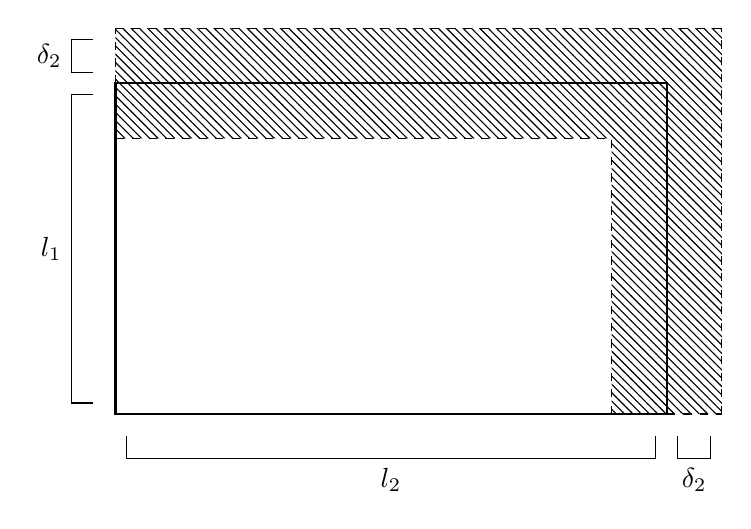
\begin{tikzpicture}[scale=1.4]
		\draw [thick](0,0)rectangle(5,3);
		\draw  (0.1,-0.2) --++(0,-0.2) --++ (4.8,0) node[pos=0.5, below] {$l_{2}$} --++(0,0.2);
		\draw [dashed](0,2.5)--(4.5,2.5);
		\draw [dashed](4.5,0)--(4.5,2.5);
		\draw [dashed](0,3.5)--(5.5,3.5);
		\draw [dashed](5.5,0)--(5.5,3.5);
		\draw [dashed](5,0)--(5.5,0);
		\draw [dashed](0,3)--(0,3.5);

		\draw (5.1,-0.2)--++(0,-0.2)--++(0.3,0)node[pos=0.5, below] {$\delta_{2}$} --++(0,0.2);
		\draw (-0.2, 0.1)--++(-0.2, 0)--++(0, 2.8) node[pos=0.5, left]{$l_1$}--++(0.2, 0);
		\draw (-0.2, 3.1)--++(-0.2, 0)--++(0, 0.3) node[pos=0.5, left]{$\delta_2$}--++(0.2, 0);
		\fill [pattern = north west lines, stroke=none](0,2.5)--++(0,1)--++(5.5,0)--(5.5,0) --++(-1,0)--++(0,2.5)--cycle;
	\end{tikzpicture}
\end{center}
L'area \tikz[scale = 0.5]\draw [pattern = north west lines](0,0)rectangle(1,1); è \underline{il doppio dell'errore assoluto sulla misura del rettangolo}.

\begin{align*}
	\delta_{rel}A = \frac{\text{ Area \tikz[scale = 0.5]\draw [pattern = north west lines](0,0)rectangle(1,1);}}{2 l_1 l_2} & = \left(l_1 + \delta_1\right) \left(l_2 + \delta_2\right) - \left(l_1-\delta _1\right)\left(l_2 - \delta _2\right) \\
	                                                                                                                        & = \frac{2 l_1 \delta_1 + 2 l_2 \delta_2}{2 l_1 l_2} = \frac{\delta_1}{ l_1} + \frac{ \delta_2}{l_2}                \\
	                                                                                                                        & = \delta_{\text{rel}}l_2 + \delta_{\text{rel}}l_1
\end{align*}
\begin{tcolorbox}
	\underline{Nota bene}: tutti questi calcoli sull'incertezza sono troppo laboriosi per i problemi. Per questo quando si calcola un risultato di un problema si esprime \underline{con tante cifre significative quante il dato iniziale che ne ha meno}
\end{tcolorbox}

\section{Relazioni tra grandezze fisiche}
Uno degli obiettivi della fisica è cercare relazioni tra grandezze, ossia formule che, calcolate su dati che inserisco io, mi permettano di ottenere altri dati. Ad esempio, la formula $ A = l^2  $  mi permette di calcolare l'area di un quadrato inserendo l'area all'interno di essa
\begin{definizione}{Variabili dipendenti e indipendenti}
	Una \underline{variabile indipendente} è una variabile in una formula che è "inserita" dallo sperimentatore (es $ l $).
	\vskip3mm
	Una \underline{variabile dipendente} è una variabile il cui valore dipende da una o più variabili indipendenti (es $ A $).
\end{definizione}
Vi sono diversi modi secondo cui una variabile può  dipendere da un'altra:
\subsection{Tipi di relazioni}
\begin{definizione}{Relazione lineare}
	Due grandezze sono in relazione lineare quando sono legate da un'equazione del tipo:
	\[
		y = kx + q
	\]
	dove q e $ k $ sono costanti
	\vskip3mm
	\begin{minipage}[c]{0.48\textwidth}
		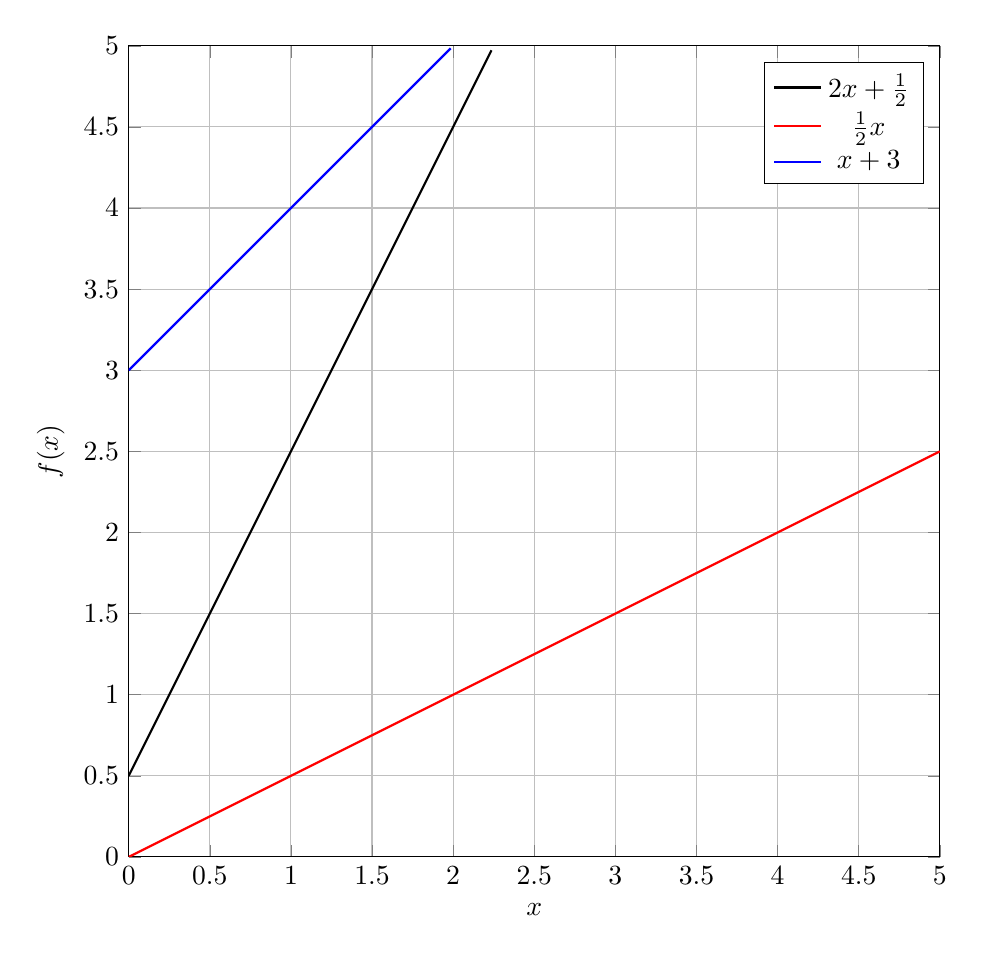
\begin{tikzpicture}
			\begin{axis}[
					xmin=0, xmax=5,
					ymin=0,ymax=5,
					restrict y to domain = 0:5, domain=0:5, width=0.98\textwidth, height=0.98\textwidth, grid=major, samples=200,  ylabel=$f(x)$, xlabel=$x$, legend entries={$2x + \frac{1}{2} $, $ \frac{1}{2}x $, $ x + 3 $}]
				\addplot[black, thick] {2*x + 0.5};
				\addplot[red, thick] {1/2*x + 0};
				\addplot[blue, thick] {x + 3};
			\end{axis}
		\end{tikzpicture}
	\end{minipage}
	%
	\begin{minipage}[c]{0.48\textwidth}
		\begin{itemize}
			\item $ q $ è l'altezza del punto in cui la retta interseca l'asse y
			\item $ k $ determina quanto la retta è "ripida"
		\end{itemize}
	\end{minipage}
\end{definizione}
Ad esempio, vi è una relazione lineare fra il volume contenuto in una caraffa e il suo peso (all'aumentare del volume aumenta il peso linearmente)
\begin{tcolorbox}
	Se due variabili sono in realzione lineare e la loro equazione ha $ q=0 $ allora si dice che fra queste vige una \underline{proporzionalità diretta}
\end{tcolorbox}

\begin{definizione}{Proporzionalità quadratica diretta}
	Due grandezze sono in relazione quadratica diretta quando sono legate da un'equazione del tipo:
	\[
		y = k \cdot x^2
	\]
	dove $ k $ è una costante
	\vskip3mm
	\begin{minipage}[c]{0.48\textwidth}
		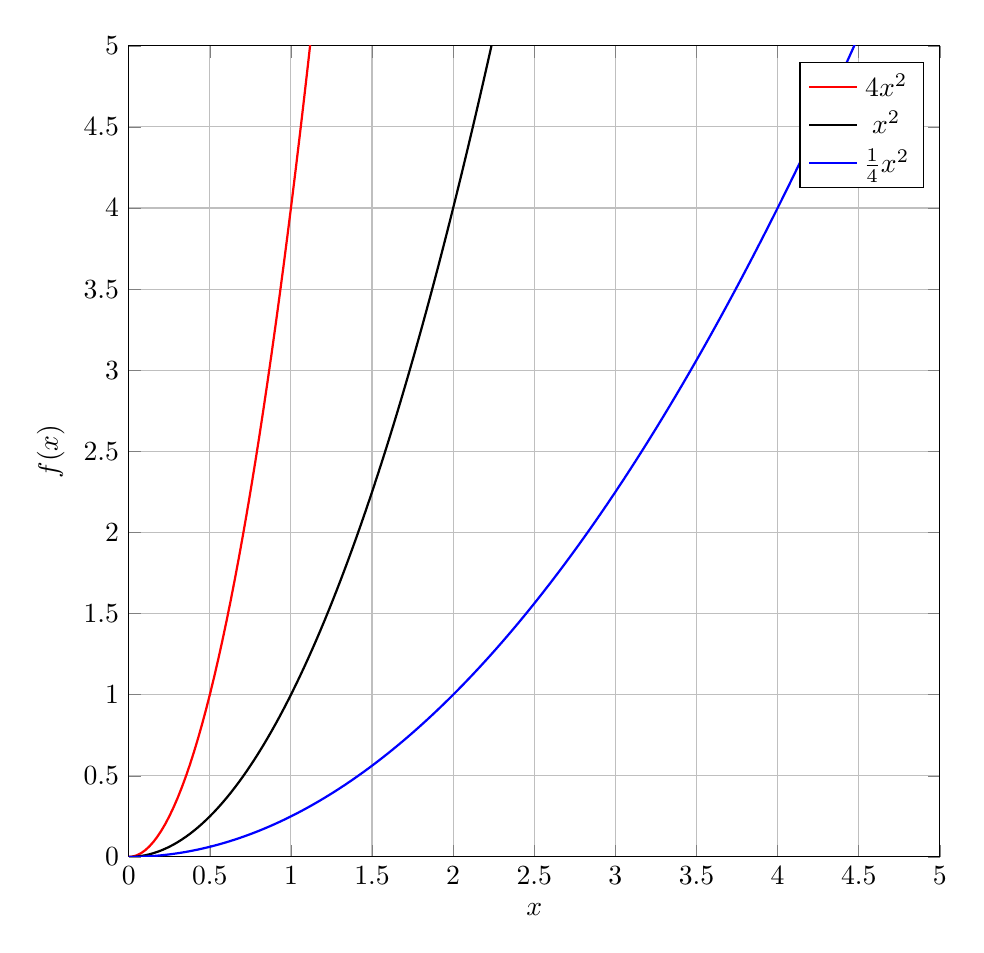
\begin{tikzpicture}
			\begin{axis}[
					xmin=0, xmax=5,
					ymin=0,ymax=5,
					restrict y to domain = 0:10, domain=0:5, width=0.98\textwidth, height=0.98\textwidth, grid=major, samples=200,  ylabel=$f(x)$, xlabel=$x$, legend entries={$ 4x^2  $, $ x^2 $, $ \frac{1}{4} x^2  $}]
				\addplot[red, thick] {4*x^2};
				\addplot[black, thick] {x^2};
				\addplot[blue, thick] {1/4* x ^2};
			\end{axis}
		\end{tikzpicture}
	\end{minipage}
	%
	\begin{minipage}[c]{0.48\textwidth}
		\begin{itemize}
			\item $ k $ determina quanto la curva "si alza velocemente"
		\end{itemize}
	\end{minipage}
\end{definizione}
Ad esempio, vi è una relazione di proporzionalità quadratica diretta fra il lato di un quadrato e la sua area: $ A = l^2 $
\begin{definizione}{Proporzionalità radicale diretta}
	Due grandezze sono in relazione di proporzionalità radicale diretta quando sono legate da un'equazione del tipo:
	\[
		y = k \sqrt{x}
	\]
	dove $ k $ è una costante
	\vskip3mm
	\begin{minipage}[c]{0.48\textwidth}
		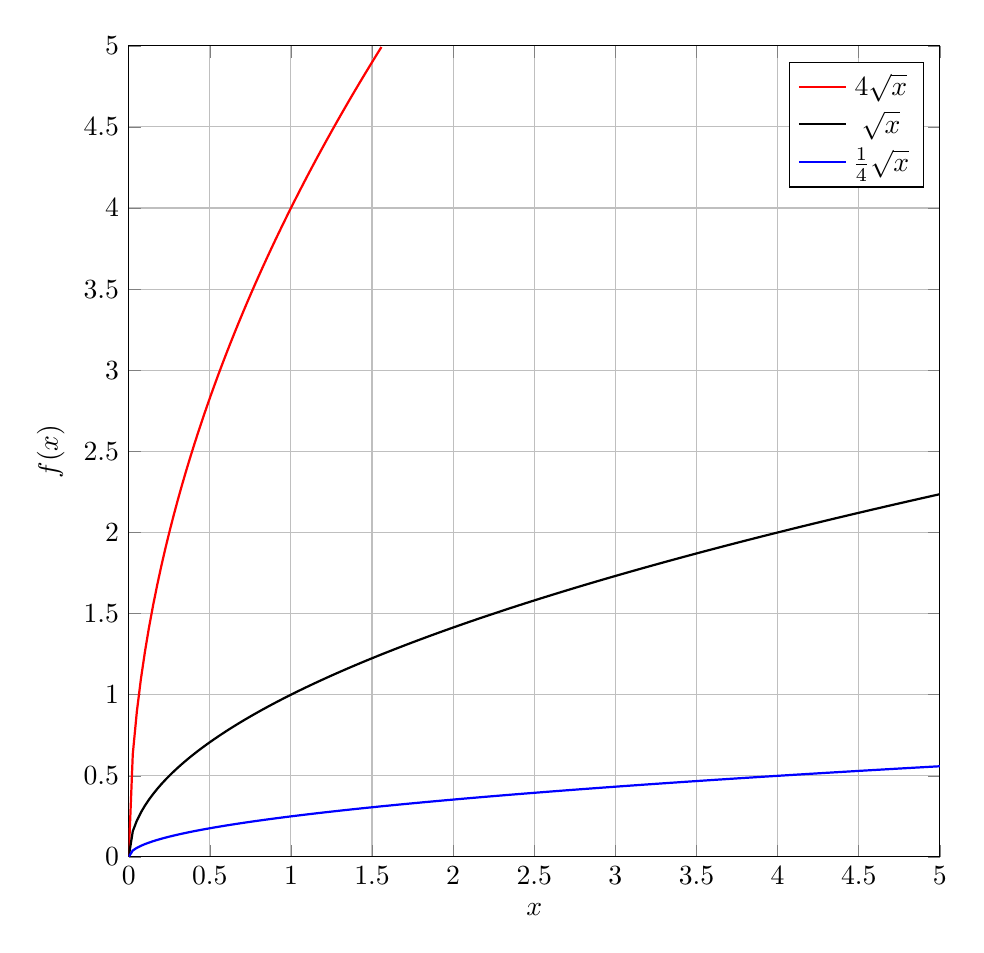
\begin{tikzpicture}
			\begin{axis}[
					xmin=0, xmax=5,
					ymin=0,ymax=5,
					restrict y to domain = 0:5, domain=0:5, width=0.98\textwidth, height=0.98\textwidth, grid=major, samples=200,  ylabel=$f(x)$, xlabel=$x$, legend entries={$ 4\sqrt{x} $, $ \sqrt{x} $, $ \frac{1}{4}\sqrt{x} $}]
				\addplot[red, thick] {4*sqrt(x)};
				\addplot[black, thick] {sqrt(x)};
				\addplot[blue, thick] {1/4* sqrt(x)};
			\end{axis}
		\end{tikzpicture}
	\end{minipage}
	%
	\begin{minipage}[c]{0.48\textwidth}
		\begin{itemize}
			\item $ k $ determina quanto la curva "si alza velocemente"
		\end{itemize}
	\end{minipage}
\end{definizione}
Ad esempio, vi è una relazione di proprorzionalità radicale fra area di un quadrato e lato: $ l = \sqrt{A} $
\begin{definizione}{Proporzionalità inversa}
	Due grandezze sono in relazione di proporzionalità inversa quando sono legate da un'equazione del tipo:
	\[
		y = \frac{k}{x}
	\]
	dove $ k $ è una costante
	\vskip3mm
	\begin{minipage}[c]{0.48\textwidth}
		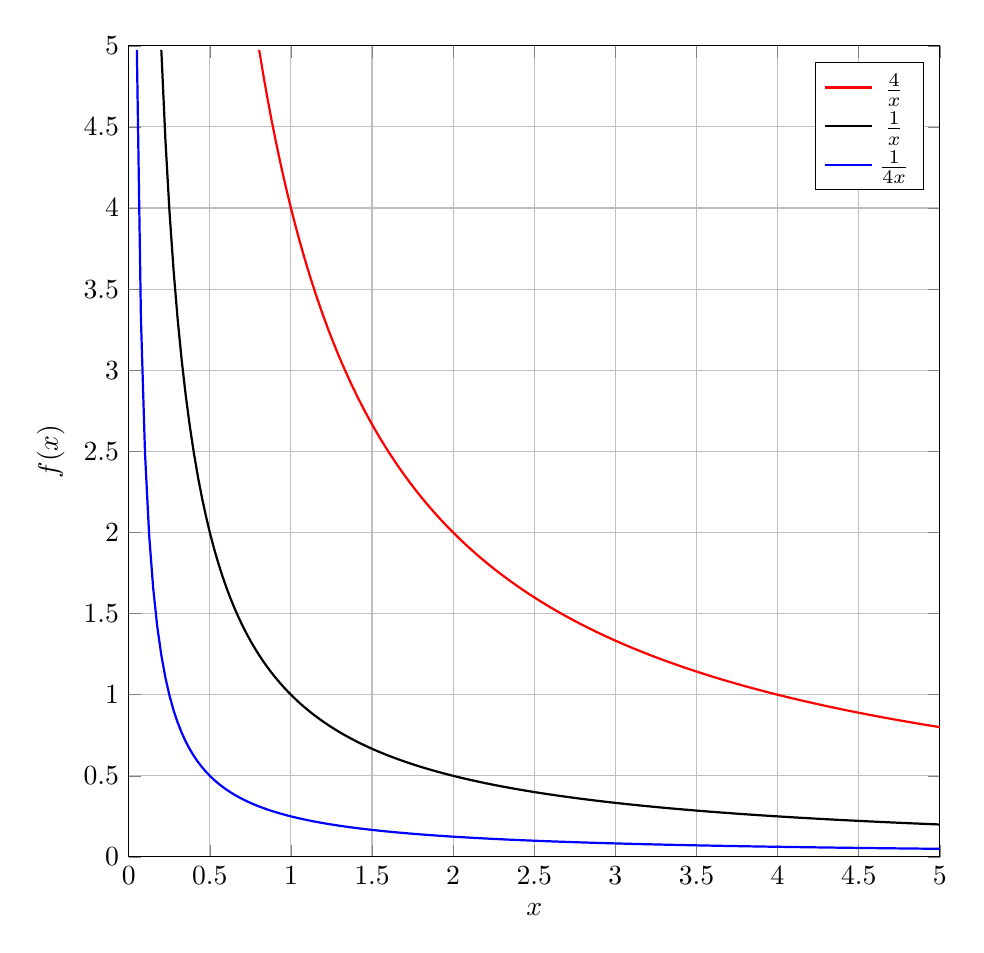
\begin{tikzpicture}
			\begin{axis}[
					xmin=0, xmax=5,
					ymin=0,ymax=5,
					restrict y to domain = 0:5, domain=0:5, width=0.98\textwidth, height=0.98\textwidth, grid=major, samples=200,  ylabel=$f(x)$, xlabel=$x$, legend entries={$ \frac{4}{x} $, $ \frac{1}{x} $, $ \frac{1}{4x} $}]
				\addplot[red, thick] {4/x};
				\addplot[black, thick] {1/x};
				\addplot[blue, thick] {1/(4 * x)};
			\end{axis}
		\end{tikzpicture}
	\end{minipage}
	%
	\begin{minipage}[c]{0.48\textwidth}
		\begin{itemize}
			\item $ k $ determina quanto la curva "si schiaccia" contro l'origine
		\end{itemize}
	\end{minipage}
\end{definizione}
Un esempio può essere il tempo necessario ad un veicolo per percorrere una determinata distanza: $ t = \frac{d}{v} $

\begin{itemize}
	\item Cosa succede quanto mi avvicino a 0 sull'asse x?
	\item Cosa succede invece quando sull'asse x vado verso valori molto grandi?
\end{itemize}
\section{Vettori}
Per rappresentare una forza i numeri non bastano in quanto dobbiamo avere modo di rappresentarne anche direzione e verso. Per questo scopo esistono \underline{i vettori}.
\begin{center}
	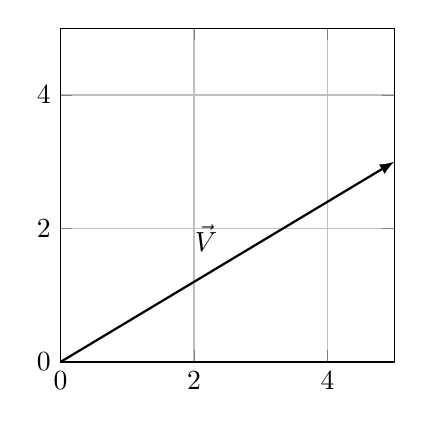
\begin{tikzpicture}
		\begin{axis}[
				xmin=0, xmax=5,
				ymin=0,ymax=5,
				restrict y to domain = 0:5, domain=0:5, width=0.48\textwidth, height=0.48\textwidth, grid=major]
			\draw [-latex, thick](0,0)--(5,3) node[pos=0.5, anchor = south east]{$ \vec{V} $};
		\end{axis}
	\end{tikzpicture}
\end{center}
\subsection{Operazioni}
\subsubsection{Addizione}
Se i vettori hanno la stessa direzione, il vettore risultante sarà un vettore con stessa direzione e modulo uguale alla somma dei moduli.
\vskip3mm
\begin{minipage}[c]{0.48\textwidth}
	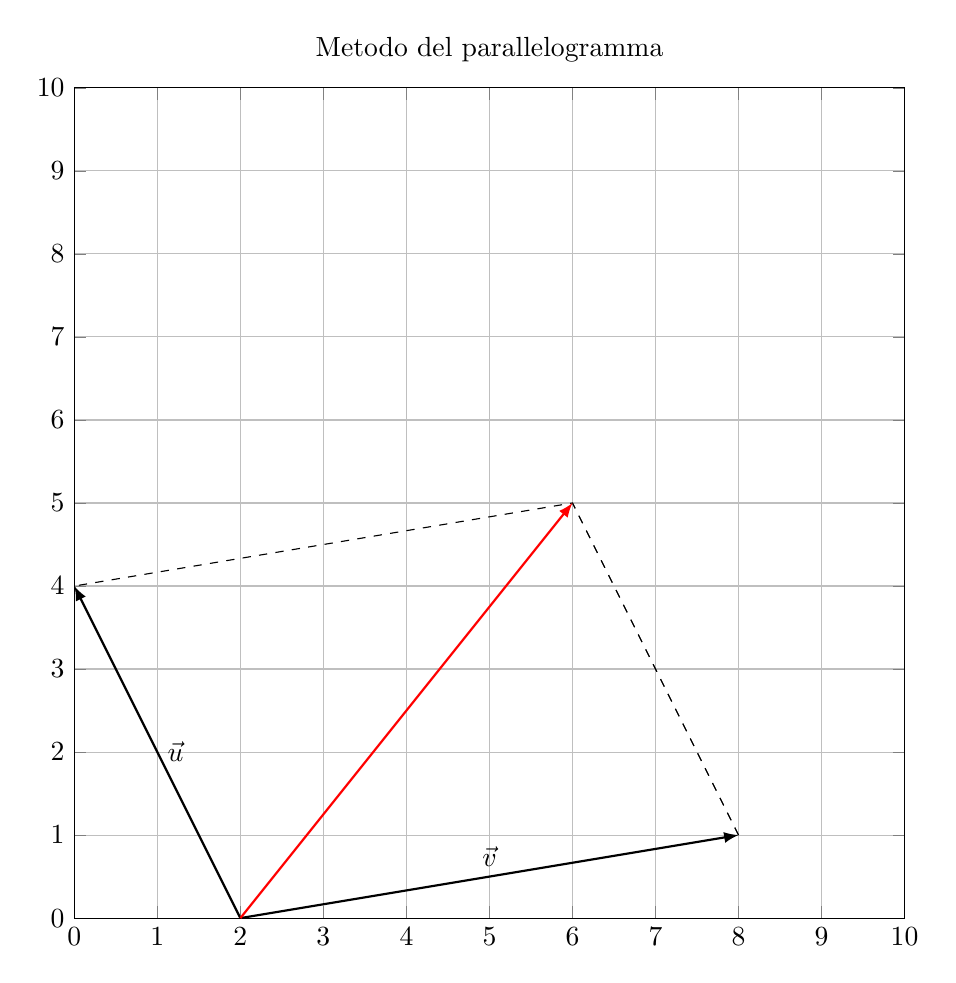
\begin{tikzpicture}
		\begin{axis}[
				title = Metodo del parallelogramma,
				xmin=0, xmax=10,
				ymin=0,ymax=10,
				restrict y to domain = 0:10, domain=0:10, width=\textwidth, height=\textwidth, grid=major]
			\draw [thick, -latex](2,0)--(8,1) node[midway, above]{$ \vec{v} $};
			\draw [thick, -latex](2,0)--(0,4) node[midway, right]{$ \vec{u} $};

			\draw [dashed](8,1)--(6,5);
			\draw [dashed](8,1)--(6,5)--(0,4);

			\draw [thick, -latex, red](2,0)--(6,5);
		\end{axis}
	\end{tikzpicture}
\end{minipage}
%
\begin{minipage}[c]{0.48\textwidth}
	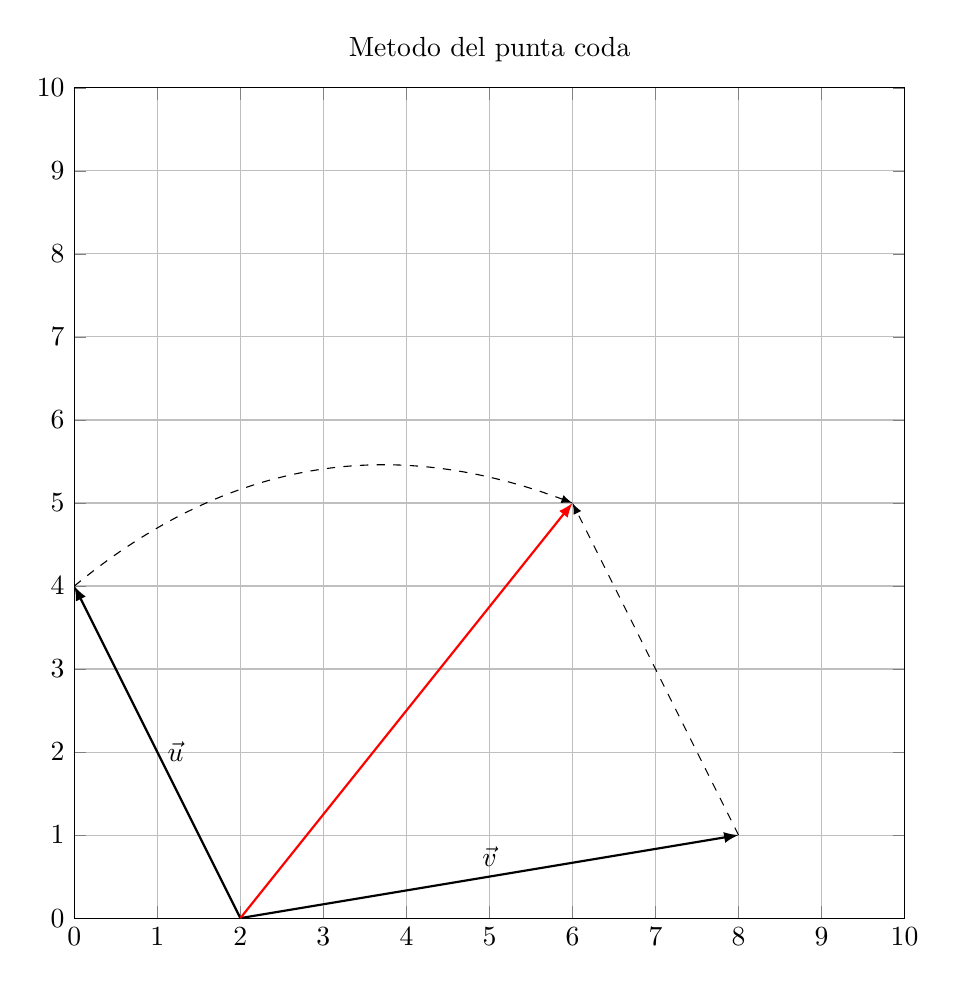
\begin{tikzpicture}
		\begin{axis}[
				title = Metodo del punta coda,
				xmin=0, xmax=10,
				ymin=0,ymax=10,
				restrict y to domain = 0:10, domain=0:10, width=\textwidth, height=\textwidth, grid=major]
			\draw [thick, -latex](2,0)--(8,1)node[midway, above]{$ \vec{v} $};
			\draw [thick, -latex](2,0)--(0,4)node[midway, right]{$ \vec{u} $};

			\draw [dashed, -latex](8,1)--(6,5);
			\draw [dashed, bend left, -latex](0,4) to (6,5);

			\draw [thick, -latex, red](2,0)--(6,5);
		\end{axis}
	\end{tikzpicture}
\end{minipage}
\vskip3mm
\underline{Somma per via grfica:}
\begin{itemize}
	\item \underline{Parallelogramma}: posiziona i due vettori in maniera tale che i punti di applicazione coincidano ("culo a culo"), completa il parallelogramma e traccia la diagonale. La diagonale è il vettore risultante
	\item \underline{Punta coda}: posiziona i due vettori in maniera tale che una delle due punte coincidano con una delle due teste e unisci le due estremità
\end{itemize}
\underline{Somma per via algebrica:}
\begin{itemize}
	\item Scomporre il vettore in componenti lungo un sistema di riferimento cartesiano come indicato in \cref{scomposizionevettori}
	\item Addizionare le componenti ottenute su asse y e x
	\item Sui due vettori ottenuti sommando le componenti, usare il teorema di pitagora per ottenere il modulo la trigonometria per ottenere direzione e verso del risultato
\end{itemize}
\subsubsection{Moltiplicazione per scalare}
La moltiplicazione per scalare $ k \vec{v} $ (per un numero), da come risultato un vettore che ha:
\begin{itemize}
	\item Direzione uguale a $ \vec{v} $
	\item Modulo uguale a $ k \cdot \left|\vec{v}\right| $
	\item Verso uguale a $ \vec{v} $ se $ k $ è positivo, invertito altrimenti
\end{itemize}

\vskip3mm
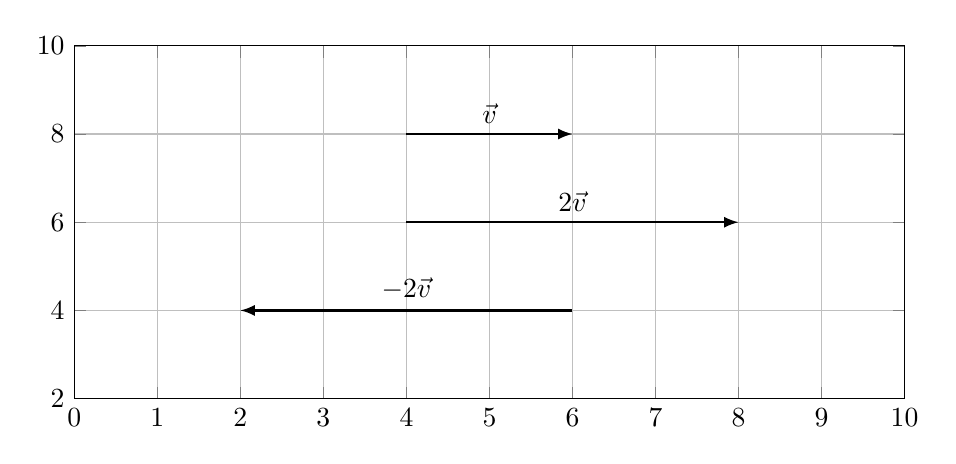
\begin{tikzpicture}
	\begin{axis}[
			xmin=0, xmax=10,
			ymin=2,ymax=10,
			restrict y to domain = 0:10, domain=0:10, width=\textwidth, height=0.5\textwidth, grid=major]
		\draw [thick, -latex](4,8)--(6,8)node[midway, above]{$ \vec{v} $};
		\draw [thick, -latex](4,6)--(8,6)node[midway, above]{$ 2 \vec{v} $};
		\draw [thick, -latex](6,4)--(2,4)node[midway, above]{$ -2\vec{v} $};
	\end{axis}
\end{tikzpicture}
\vskip3mm
\subsubsection{Sottrazione}
Per effettuare la sottrazione si può applicare l'addizione sul secondo vettore moltiplicato per lo scalare $ -1 $ ($ \vec{v} - \vec{u} = \vec{v} + \left(-\vec{u}\right) $). Questo, graficamente, coincide con :
\begin{itemize}
	\item Mettere i vettori in maniera tale che i punti di applicazione coincidano
	\item Congiungere l'estremità del vettore sottrato con quello dal quale lo stiamo sottraendo
\end{itemize}
\vskip3mm
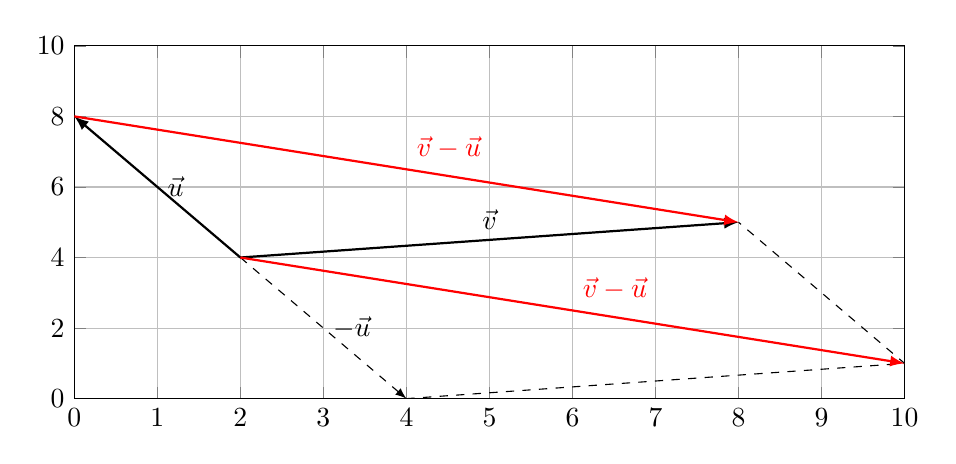
\begin{tikzpicture}
	\begin{axis}[
			xmin=0, xmax=10,
			ymin=0,ymax=10,
			restrict y to domain = 0:10, domain=0:10, width=\textwidth, height=0.5\textwidth, grid=major]
		\begin{scope}[shift={(0,4)}]
			\draw [thick, -latex](2,0)--(8,1)node[midway, above]{$ \vec{v} $};
			\draw [thick, -latex](2,0)--(0,4)node[midway, right]{$ \vec{u} $};
		\end{scope}
		\draw [dashed, -latex](2,4)--(4,0) node[midway, right]{$ -\vec{u} $};
		\draw [dashed](4,0) -- (10,1) -- (8,5);
		\draw [thick, -latex, red](2,4)--(10,1)node[midway, right, anchor = south west]{$ \vec{v}-\vec{u} $};
		\draw [thick, -latex, red](0,8)--(8,5)node[midway, right, anchor = south west]{$ \vec{v}-\vec{u} $};
	\end{axis}
\end{tikzpicture}
\subsubsection{Prodotto scalare}
Si indica con il pallino $ \cdot  $ da come risultato uno scalare (un numero) uguale a $ \left|\vec{v}\right| \left|\vec{u}\right| \cos \left(\alpha \right) $ dove $ \alpha  $ è \underline{l'angolo compreso} tra $ \vec{v} $ e $ \vec{u} $
\vskip3mm
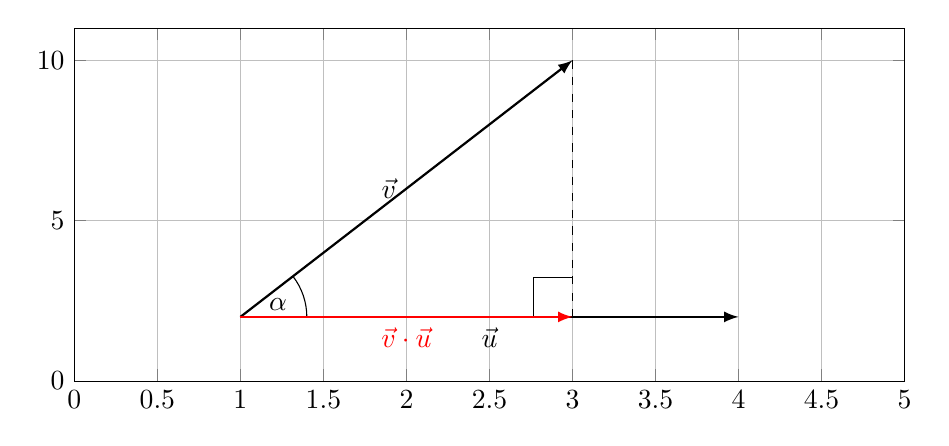
\begin{tikzpicture}
	\begin{axis}[
			xmin=0, xmax=5,
			ymin=0,ymax=11,
			restrict y to domain = 0:10, domain=0:10, width=\textwidth, height=0.5\textwidth, grid=major]
		\coordinate (a) at (1,2);
		\coordinate (b) at (3,10);
		\coordinate (c) at (4,2);
		\coordinate (int) at (3,2);
		\draw [thick, -latex](a)--(b)node[midway, left]{$ \vec{v} $};;
		\draw [thick, -latex](a)--(c)node[midway, below]{$ \vec{u} $};;
		\draw [dashed](b)--(3,2);
		\pic [draw, "$ \alpha $", angle radius = 24] {angle = c--a--b};
		\pic [draw] {right angle = b--int--a};
		\draw [thick,  -latex, red](a) -- (int)node[midway, below]{$ \vec{v} \cdot \vec{u} $};;
	\end{axis}
\end{tikzpicture}
\subsubsection{Prodotto vettoriale}
\label{prodvettoriale}
Si indica con la croce $ \times  $  e da come risultato \underline{un vettore} che abbia
\begin{itemize}
	\item Direzione perpendicolare al piano che contiene $ \vec{v} $ e $ \vec{u} $
	\item Modulo uguale a $ \left|\vec{v}\right| \left|\vec{u}\right|\sin \left(\alpha \right) $ dove $ \alpha  $ è l'angolo compreso tra $ \vec{v} $ e $ \vec{u} $
	\item Direzione data dalla regola della mano destra:
	      \begin{itemize}
		      \item Dato $ \vec{v} \times \vec{u} $, posizionare pollice sul primo vettore
		      \item Posizionare l'indice sul secondo
		      \item La direzione del palmo costituisce da direzione del vettore risultante
	      \end{itemize}
\end{itemize}
\vskip3mm
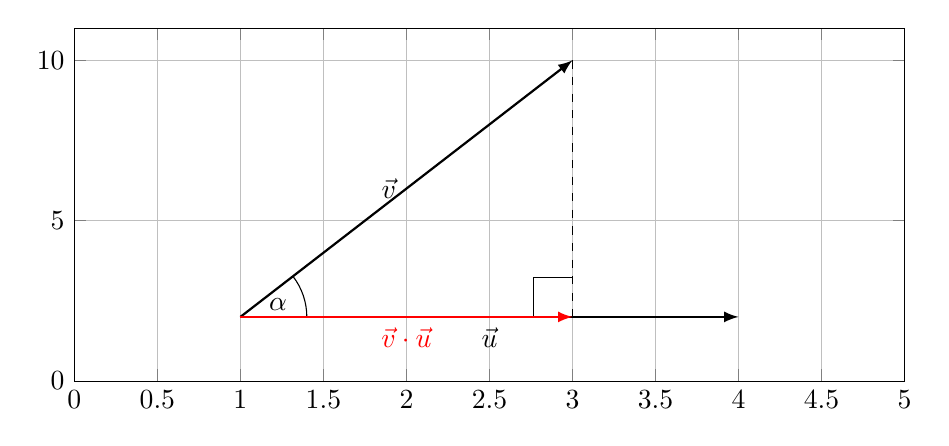
\begin{tikzpicture}
	\begin{axis}[
			xmin=0, xmax=5,
			ymin=0,ymax=11,
			restrict y to domain = 0:10, domain=0:10, width=\textwidth, height=0.5\textwidth, grid=major]
		\coordinate (a) at (1,2);
		\coordinate (b) at (3,10);
		\coordinate (c) at (4,2);
		\coordinate (int) at (3,2);
		\draw [thick, -latex](a)--(b)node[midway, left]{$ \vec{v} $};;
		\draw [thick, -latex](a)--(c)node[midway, below]{$ \vec{u} $};;
		\draw [dashed](b)--(3,2);
		\pic [draw, "$ \alpha $", angle radius = 24] {angle = c--a--b};
		\pic [draw] {right angle = b--int--a};
		\draw [thick,  -latex, red](a) -- (int)node[midway, below]{$ \vec{v} \cdot \vec{u} $};;
	\end{axis}
\end{tikzpicture}

\subsection{Scomposizione}\label{scomposizionevettori}
Scomporre un vettori lungo assi di un sistema di riferimento cartesiano risulta cruciale nella risoluzione di problemi di statica. Un sistema di riferimento cartesiano non è altro che due assi perpendicolari fra di loro.
\vskip3mm
L'idea della scomposizione di un vettore è trovare due vettori lungo gli assi che sommati diano il vettore di partenza:

\vskip3mm
\begin{center}
	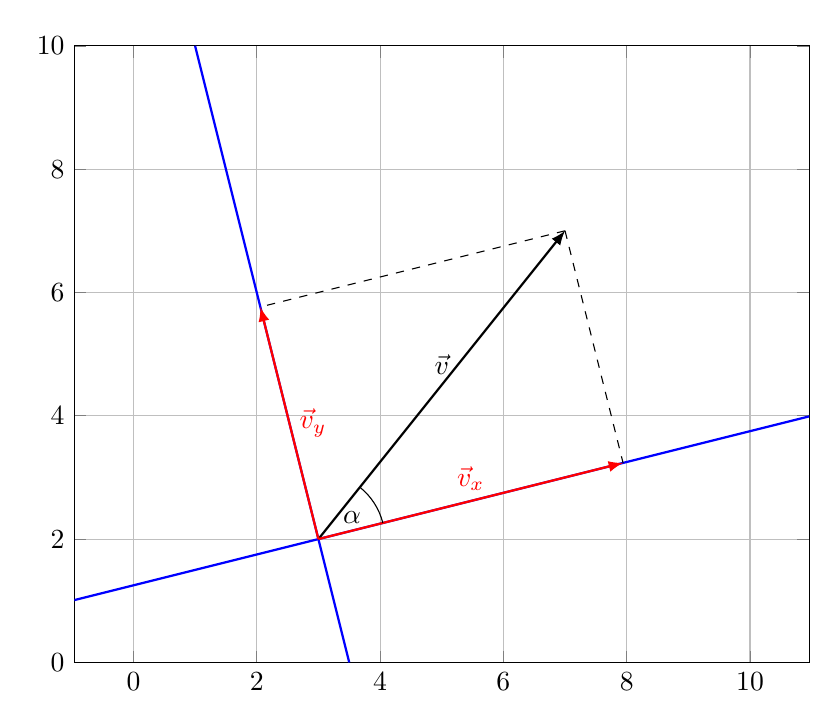
\begin{tikzpicture}
		\begin{axis}[
				axis equal,
				xmin=0, xmax=10,
				ymin=0,ymax=10,
				restrict y to domain = 0:10, domain=0:10, width=0.9\textwidth, grid=major]
			\coordinate (o) at (3,2);
			\coordinate (xaxis) at (11,4);
			\coordinate (yaxis) at (3.5,0);
			\coordinate(v) at (7,7);
			%
			\draw [blue, thick](1,10)--(3.5,0);
			\draw [blue, thick](-1,1)--(11,4);
			%
			\draw [dashed](v)--($(o)!(v)!(xaxis)$);
			\draw [dashed](v)--($(o)!(v)!(yaxis)$);

			\draw [thick, -latex](o)--(v)node[midway, above]{$ \vec{v} $};

			\draw [thick, -latex, red](o)--($(o)!(v)!(xaxis)$)node[midway, above]{$ \vec{v}_{x} $};
			\draw [thick, -latex, red](o)--($(o)!(v)!(yaxis)$) node[midway, right]{$ \vec{v}_{y} $};
			%
			\pic [draw,  "$ \alpha $", angle radius = 24pt] {angle = xaxis--o--v};
		\end{axis}
	\end{tikzpicture}
\end{center}

\subsection{Trigonometria}\label{trigonometria}
Per scomporre un vettore sono necessarie alcune nozione sugli angoli rettangoli:
\vskip3mm
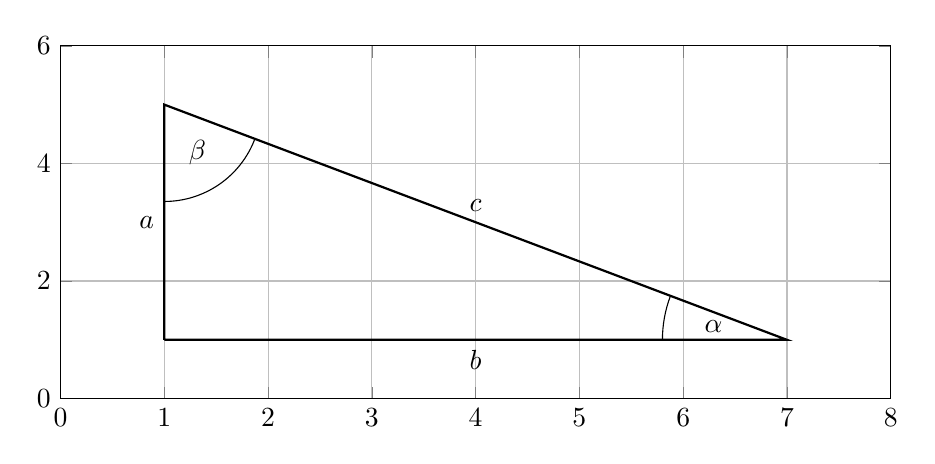
\begin{tikzpicture}
	\begin{axis}[
			xmin=0, xmax=8,
			ymin=0,ymax=6,
			restrict y to domain = 0:10, domain=0:10, width=\textwidth, height=0.5\textwidth, grid=major]
		\coordinate (a) at (1,1);
		\coordinate (b) at (7,1);
		\coordinate (c) at (1,5);
		%
		%
		%
		\draw [thick](a)--(b)node[midway, below] {$ b $}
		--(c)node[midway, above] {$ c $}
		--(a)node[midway, left] {$ a $};
		\pic [draw,  "$ \alpha $", angle radius = 45pt] {angle = c--b--a};
		\pic [draw,  "$ \beta  $", angle radius = 35pt] {angle = a--c--b};
	\end{axis}
\end{tikzpicture}
\vskip3mm
\begin{itemize}
	\item Ipotenusa $ \Leftrightarrow $ cateto
	      \begin{align*}
		      \text{ cateto } & = \text{ ipotenusa } \cdot \text{ seno angolo opposto a cateto che voglio calcolare }
		      \text{ cateto } & = \text{ ipotenusa } \cdot \text{ coseno angolo adiacente a cateto che voglio calcolare }
	      \end{align*}
	      nel nostro caso abbiamo che:
	      \begin{align*}
		      a & = c \cdot \sin  \alpha = c \cdot  \cos \beta  \\
		      b & = c \cdot \cos   \alpha = c \cdot  \sin \beta \\
	      \end{align*}
	\item Cateto $ \Leftrightarrow $ cateto
	      \[
		      \text{ cateto 1 } = \text{ cateto 2 } * \tan \text{ angolo adiacente a cateto 2 }
	      \]
	      nel nostro caso:
	      \begin{align*}
		      a & = b \tan \alpha \\
		      b & = a \tan \beta
	      \end{align*}
	\item Cateti $ \Rightarrow $ ipotenusa: si usa il teorema di Pitagora
	      \begin{align*}
		      \text{ (ipotenusa) } ^2 & = \text{ (cateto 1)} ^2 + \text{ (cateto 2) } ^2        \\
		      \text{ (ipotenusa) }    & = \sqrt{\text{ (cateto 1)} ^2 + \text{ (cateto 2) } ^2}
	      \end{align*}
	      nel nostro caso
	      \begin{align*}
		      c = \sqrt{a ^2  + b ^2 }
	      \end{align*}
\end{itemize}

\section{Statica}
La statica si occupa dello studio di fenomeni per l'appunto statici. L'idea è di prendere un sistema di nostra interesse, "scattare una fotografia" e studiare le forze che agiscono su di esso.
\subsection{Forze}
Vediamo ora le pricipali forze
\subsubsection{Forza peso}
E' la forza provocata dalla gravità. Va fatta la distinzione fra peso e massa :
\begin{itemize}
	\item \underline{Massa}: è una proprietà instrinseca di un oggetto, in un certo senso decreta la quantità di materia che possiede, non dipende dal "pianeta". Si misura in kg
	\item \underline{Peso}: è la forza che un oggetto dotato di massa subisce quando è in un campo gravitazionale. Dipende dal pianeta e si misura in N
\end{itemize}
Quando si parla di forze bisogna sempre convertire i kg in N. Per farlo basta la seguente formula:
\[
	\text{ peso } = \text{ massa } \cdot \text{ costante gravitazionale ($ g $)}
\]
se siamo sulla terra, la \textit{costante gravitazionale} vale 9.81. Es
\[
	5 \left[\text{ kg }\right] = 5 \left[\text{ kg }\right] \cdot 9.81 \left[\frac{\text{ N }}{\text{ kg }}\right] \approx 49 \left[\text{ N }\right]
\]

\subsubsection{Forza elastica}
E' la forza esercitata da un oggetto che spostato dalla sua posizione di riposo, vuole tornarci. Tendenzialmente, si parla di molle. La forza esercitata da una molla è data dalla legge di hooke:
\[
	F_{e} = k \cdot \Delta x
\]
dove $ k $ è la costate di Hooke, che indica "quanto la molla è dura" e $ \Delta x $ è l'allungamento della molla rispetto alla posizione di riposo
\subsubsection{Reazione vincolare}
Immaginiamo di appoggiare un libro su un tavolo. Il libro non "sprofonda" nel tavolo in quanto il tavolo esercita su di esso una forza uguale e contraria. Tale forza è detta \underline{reazione vincolare}. Questa forza è uguale alla componente parallela di tutte le forze che vengono esercitate su di una superficie:
\vskip3mm
\begin{center}
	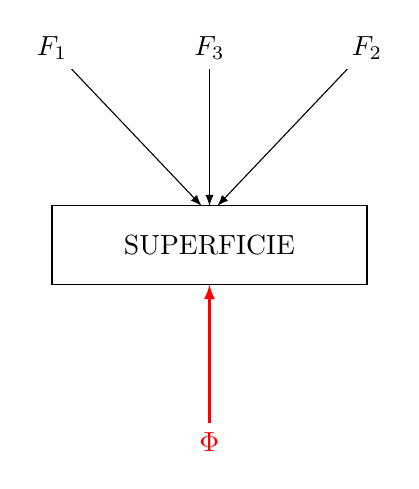
\begin{tikzpicture}
		\draw (-2,0)rectangle(2,-1);
		\node at (0, -0.5) {SUPERFICIE};
		\draw [-latex](-2,2)node[fill = white]{$ F_1 $}--(-0.1,0);
		\draw [-latex](2,2)node[fill = white]{$ F_2 $}--(0.1,0);
		\draw [-latex](0,2)node[fill = white]{$ F_3 $}--(0,0);
		\draw [thick,-latex, red](0,-3)node[fill = white]{$ \Phi $}--(0,-1);
	\end{tikzpicture}
\end{center}
\subsubsection{Forza d'attrito}
La forza d'attrito è data dalla scabrosità di un materiale.
\[
	F_s = \mu _s \cdot  \Phi
\]
dove $ \mu _s $ è il \textit{coefficiente d'attrito}, ossia una costante tabellare che dipende dalle caratteristiche fisiche dei materiali a contatto e $ \Phi  $ è la reazione vincolare che la soperficie esercita sull'oggetto appoggiato

\subsection{Equilibrio dei corpi rigidi}
Prendiamo il seguente problema di statica:
\vskip3mm
\begin{center}
	\begin{tikzpicture}
		\draw (0,0)rectangle(5,1);
		\draw [-latex](0.5,-1) --(0.5,0)node [midway, anchor = west]{$ \vec{F_1} $};
		\draw [-latex](4.5,2)--(4.5,1)node [midway, anchor = west]{$ \vec{F_2} $};
	\end{tikzpicture}
\end{center}
\vskip3mm
Se $ \left|F_1\right| = \left|F_2\right| $ secondo ciò che abbiamo detto fin'ora il corpo dovrebbe essere in equilibrio e non dovrebbe quindi non compiere nessun movimento. L'esperienza di tutti i giorni è in constrasto con ciò (il corpo ruota in direzione oraria).
\vskip3mm
Questo succede perché abbiamo trattato i corpi come \underline{punti materiali}, ossia potevamo semplificare il sistema immaginandoci il corpo come un minoscolo pallino sul quale le forze agiscono tutte nello stesso punto. Per corpi estesi bisogna invece tenere conto del fatto che questi possano anche \underline{ruotare}

\subsubsection{Momento torcente}
Per parlare di rotazione in fisica è fondamentale aver chiaro il concetto di momento. In particolare, una forza che tende a far ruotare un oggetto genera un \underline{momento torcente}, che esprime \textit{"l'intensità con la quale l'oggetto vuole girare per effetto della medesima forza"}. Supponiamo di avere un bastone ancorato ad un'estemità:
\begin{center}
	\begin{tikzpicture}
		\draw (0,-0.5)rectangle(5,0.5);
		\draw [fill = white](0,0)circle(0.5);
		\draw [-latex](4.5,2)--(4.5,1)node [midway, anchor = west]{$ \vec{F} $};
	\end{tikzpicture}
\end{center}
per descrivere la rotazione indotta da $ \vec{F} $ è necessario indicare:
\begin{itemize}
	\item La \textit{direzione} della rotazione (senso orario o antiorario)
	\item L'intensità della torsione (ad esempio quanto forte serve girare per aprire una bottiglia)
\end{itemize}

Per descrivere ciò si usano i momenti. In particolare, data una forza $ \vec{F} $, il suo momento torcente dato da:
\[
	\vec{M} = \vec{r} \times \vec{F} \quad  \rightarrow \quad \left|M\right| = \left|r\right| \cdot \left|F\right| \cdot \sin \left(\alpha \right)
\]

dove
\begin{itemize}
	\item $ \vec{r} $ è il vettore che congiunge il punto di applicazione della forza con il centro della rotazione
	\item $ \vec{F} $ la forza che imprime la rotazione
\end{itemize}

Attenzione che con $ \times  $ si indica il \underline{prodotto vettoriale} (vedi sez \ref{prodvettoriale})

\bigbox{
	Possiamo ora introduttre il concetto di \underline{equilibrio di corpi rigidi:}
	\vskip3mm
	Un corpo rigido è in equilibrio statico se la somma delle forze e la somma dei momenti torcenti è \underline{zero}
}

\vskip3mm
Cerchiamo ora di dare interpretazione fisica ai momenti.
\begin{itemize}
	\item \underline{Verso}:
	      Abbiamo verso entrante nel caso in cui generino una rotazine in senso \underline{orario}, mentre uscente nel caso la generino in senso \underline{antiorario}. Cio vuol dire che quando sommiamo i momenti le forze che fanno ruotare in senso orario si oppongono a quelle che fanno ruotare in senso orario, il che è ragionevole
	\item \underline{Intensità}:
	      L'intensità di un momento torcente è pari a $ \left|r\right| \cdot \left|F\right| \cdot \sin \left(\alpha \right) $. Vediamo quindi come l'intensità della torsione aumenti all'aumentare della
	      \begin{itemize}
		      \item Forza, il che è evidente
		      \item Raggio della forza: più lontano sono dal centro della rotazione, più forza applico, il che è ragionevole. Supponiamo di voler svitare un dado con una chiave inglese. Faremmo più fativa applicando la forza vicino al dado o all'estremità della chiave inglese?
		            \begin{center}
			            \begin{tikzpicture}
				            \draw (0,-0.5)rectangle(5,0.5);
				            \draw [fill = white](0,0)circle(0.5);
				            \draw [-latex](4.5,2)--(4.5,1)node [midway, anchor = west]{$ \vec{F_1} $};
				            \draw [-latex](2.5,2)--(2.5,1)node [midway, anchor = west]{$ \vec{F_2} $};
			            \end{tikzpicture}
		            \end{center}
	      \end{itemize}
\end{itemize}

\usetikzlibrary{calc}
\usetikzlibrary{intersections}

%\subsubsection{Equilibrio risivitato}
%Supponi di avere la situazione illustrata in figura: 
%\begin{center}
%  \begin{tikzpicture}
%    \coordinate (a) at (0,0);
%    \coordinate (b) at (7,0);
%    \coordinate (c) at (0,3);
%    \draw (a)--(b) -- (c) -- cycle;
%    %\node (prova)[] at (3,2.5) {prova};
%    %\draw (3,2.5)--($(c)!(3,2.5)!(b)$);
%    \coordinate (base1) at ($(b)!0.6!(c)$);
%    \coordinate (base2) at ($(b)!0.8!(c)$);
%    \coordinate (top1) at ($(base1)!0.5cm!-90:(base2)$);
%    \coordinate (top2) at ($(base2)!0.5cm!90:(base1)$);
%%
%    \path [name path = diag1] (base1)--(top2);
%    \path [name path = diag2](base2)--(top1);
%    \fill[name intersections={of=diag1 and diag2}] (intersection-1) coordinate (massCenter);
%    %\coordinate (center) at 
%    \draw (base2)--(top2)--(top1)--(base1);
%
%    \draw [-latex](massCenter)--+(0,-1);
%%
%
%%    \coordinate (p1) at ($(a)!7cm!270:(b)$);
%%    \coordinate (p2) at ($(a)!(p1)!(b)$);
%    %\node (p)[] at (p1) {p};
%    %\draw (p1)--(p2);
%\end{tikzpicture} 
%\end{center}
\subsection{Problemi}

\begin{esercizio}{Una porta}
	Per aprire una porta spingiamo in un punto a 50 mm dalle cerniere impiegando una forza 17 volte più grande di quella richiesta,se la spinta fosse fatta all'estremità libera della porta.

	\begin{center}
		\begin{tikzpicture}
			\draw (0,0)--(4,0);
			\draw [-latex](0, -1)--(0,0)node[midway, right]{$ \vec{F_1} $};
			\draw [-latex](2, -1)--(2,0)node[midway, right]{$ \vec{F_2} $};
			%
			\draw [latex-latex, dashed](2, 0.5)--(4,0.5)node[midway, above]{50 mm};
			\draw [latex-latex, dashed](0, 1)--(4,1) node [midway, above]{$ b $};
			%
			\draw [dotted](0,0)--++(0,1);
			\draw [dotted](2,0)--++(0,0.5);
			\draw [dotted](4,0)--++(0,1);
			\draw [fill = white](4,0)circle(3pt);
			\node ()[fit = (current bounding box), inner sep = 3pt] {};
		\end{tikzpicture}
	\end{center}
	Qual è la lunghezza della porta?
	\vskip3mm
	\hfill [0.85m]
\end{esercizio}

\begin{esercizio}{Due leve}
	Abbiamo una situazione come nella figura sottostante:
	\begin{center}
		\begin{tikzpicture}
			\draw (0,0)--(6,0);

			\draw [dotted, latex-latex](0,0.5)--(2,0.5)node[midway, above]{$ 160 $};
			\draw [dotted, latex-latex](2,0.5)--(6,0.5)node[midway, above]{$ 240 $};

			\draw [dotted](0,0)--++(0,0.5);
			\draw [dotted](2,0)--++(0,0.5);
			\draw [dotted](6,0)--++(0,0.5);

			\draw [fill = white](2,0)circle(3pt);
			\draw [fill = black](0,0)circle(1.5pt);
			\draw [fill = black](6,0)circle(1.5pt);

			\draw [-latex](0,0)--(0,-1) node[midway, right]{$ \vec{P} $};
			\begin{scope}[shift={(4,-2)}]
				\draw (0,0)--(6,0);

				\draw [dotted, latex-latex](0,-0.5)--(2,-0.5)node[midway, below]{$ 120 $};
				\draw [dotted, latex-latex](2,-0.5)--(6,-0.5)node[midway, below]{$ 280 $};

				\draw [dotted](0,0)--++(0,-0.5);
				\draw [dotted](2,0)--++(0,-0.5);
				\draw [dotted](6,0)--++(0,-0.5);

				\draw [fill = white](0,0)circle(3pt);
				\draw [fill = black](2,0)circle(1.5pt);
				\draw [fill = black](6,0)circle(1.5pt);

				\draw [-latex](6,0)--++(0,-1) node[midway, right]{$ \vec{F} $};
			\end{scope}

			\draw (6,0)--++(0,-2);
			\node ()[fit = (current bounding box), inner sep = 3pt] {};
		\end{tikzpicture}
	\end{center}
	Supponendo che le leve siano ancorate nei punti \underline{bianchi} e che $ \left|P\right| = 900 $, calcolare il valore di $ \left|F\right| $ affinchè il sistema rimanga in equilibrio
	\vskip3mm
	\hfill [180 N]
\end{esercizio}

\subsection{Approfondimento sulla scelta dell'origine}
Per affrontare un problema sui momento dobbiamo innanzitutto scegliere un'origine o un polo. Viene spesso detto che questo può essere scelto in modo \textit{arbitrario}, ma ciò non è vero in ogni caso:
\begin{center}
	\begin{forest}
		for tree={draw, grow = 0, align = left}
		[Scelta momento
			[Somma forze {$ = 0 $}
					[Scelgo in modo arbitrario]
			]
			[Somma forze {$ \neq 0 $}
					[Si capisce \\ punto attorno \\ al quale ruota
							[Scelgo centro \\ di rotazione]
					]
					[\underline{Non} si capisce \\ punto attorno \\ al quale ruota
							[Nulla da fare]
					]
			]
		]
	\end{forest}
\end{center}

\bigbox{Nel momento in cui scegliamo un'origine (o \textit{polo}), possiamo scegliere qualsiasi punto a patto che la risultante delle forze sul sistema sia nulla:
	\[
		\text{ scelta polo è arbitraria } \Leftrightarrow \vec{F_{tot}} = 0
	\]
}

Si può dimostrare questo come segue. Supponiamo di avere una forza e due possibili origini $ o_1 $   e $ o_2 $:
\begin{center}
	\begin{tikzpicture}[scale = 0.5]
		\coordinate (o1) at (5,1);
		\coordinate (o2) at (-1,0);
		\coordinate (v) at (3,4);
		\node [blackdot, label={0:$ o_2 $}] at (o1){};
		\node [blackdot, label={180:$ o_1 $}] at (o2){};
		\draw [-latex](v)--++(3,4)node [midway, above left]{$ \vec{F} $};
		\draw [-latex](o1)--(v) node [midway, above right]{$ \vec{b_2} $};
		\draw [-latex](o2)--(v) node [midway, above left]{$ \vec{b_1} $};
		\draw [-latex](o2)--(o1)node [midway, above left]{$ \vec{v} $};
	\end{tikzpicture}
\end{center}

\begin{itemize}
	\item Il momento della forza $ \vec{F} $ secondo $ o_1 $ è $ \vec{b_1} \times \vec{F} $
	\item Il momento della forza $ \vec{F} $ secondo $ o_2 $ è $ \vec{b_2} \times \vec{F} $
\end{itemize}
Il momento secondo $ o_2 $ può anche essere scritto in funzione di $ b_1 $ come segue :
\begin{align*}
	\vec{b_2} \times \vec{F} & = \left(\vec{b_1} - \vec{v}\right) \times \vec{F}       \\
	                         & = \vec{b_1} \times \vec{F} - \vec{v} \times  \vec{F}    \\
	                         & = M_{o_1}\left(\vec{F}\right) - \vec{v} \times  \vec{F}
\end{align*}
in quanto osservando i vettori si può vedere come $ \vec{b_2} = \vec{b_1} - \vec{v} $
Ora supponiamo di avere due forze $ F_1 $ e $ F_2 $  e di esprimere il momento totale secondo il polo $ o_2 $:
\begin{align*}
	M_{\text{tot }o_2} & = M_{F_1\;o_2} + M_{F_2\;o_2}                 \\
	                   & = b_2 \times \vec{F_1} + b_2 \times \vec{F_2}
\end{align*}
usando ora quanto ricavato pocanzi possiamo scrivere il momento come segue:
\begin{align*}
	 & = b_2 \times \vec{F_1} + b_2 \times \vec{F_2}                                                                         \\
	 & = M_{o_1}\left(\vec{F_1}\right) - \vec{v} \times \vec{F_1} + M_{o_1}\left(\vec{F_2}\right) - \vec{v} \times \vec{F_2}
\end{align*}
riordinando la formula otteniamo:
\[
	M_{\text{tot }o_2}= M_{o_1}\left(\vec{F_1}\right) + M_{o_1}\left(\vec{F_2}\right) - \vec{v} \times \vec{F_1}  - \vec{v} \times \vec{F_2}
\]
e raccogliendo $ -\vec{v} $:
\[
	M_{\text{tot }o_2} = M_{o_1}\left(\vec{F_1}\right) + M_{o_1}\left(\vec{F_2}\right) - \vec{v} \times \left(\vec{F_1}  + \vec{F_2}\right)
\]
dunque, se la \underline{somma vettoriale} delle forze è nulla, il momento totale calcolato scegliendo $ o_1 $ come polo è uguale al momento totale calcolato scegliendo $ o_2 $ come polo


%\tikzstyle{molla}=[snake = coil, segment amplitude=5, segment length=5]
%\begin{center}
%  \begin{tikzpicture}[scale = 0.7]
%		%\draw [snake = coil, segment amplitude=5, segment length=5] (0,0)--(2,2);
%		\coordinate (p1) at (0,0);
%		\coordinate (p2) at (3,0);
%		\coordinate (p3) at (7,0);
%		%
%    \draw [molla] (p1)--(p2) node [midway, above, outer sep = 5pt]{$ k_1 $};
%		\draw [molla] (p2)--(p3) node [midway, above, outer sep = 5pt]{$ k_2 $};
%    \path (p3)--++(2,2) coordinate (c2);
%		%
%		\path  [name path = 30] (p3)--($(p3) ! 10 ! -30: (8,0) $);
%		\path  [name path = wall] (p3) ++ (2,0) --++(0,4)--++(0,-8);
%		\path [name intersections={of = 30 and wall}] coordinate (c1) at (intersection-1) ;
%		\draw (c1)--(p3);
%		\draw (c2)--(p3);
%		%
%    \draw [-latex] (c1)--++(-30:1) node[midway, above] {$ \vec{F_2} $};
%		\draw [-latex] (c2)--++(45:2) node[midway, below right] {$ \vec{F_1} $};
%		%
%    \draw (p3)--++(2,0)coordinate (p);
%    \draw pic["$ \alpha_1  $", draw, angle radius = 2em] {angle = p--p3--c2};
%    \draw pic["$ \alpha_2  $", draw, angle radius = 2em] {angle = c1--p3--p};
%    %
%    \node [whitedot, label={90:$ p_1 $}] at (p2){};
%		\node [whitedot, label={90:$ p_2 $}] at (p3){};
%		\node [whitedot] at (c1){};
%		\node [whitedot] at (c2){};
%    \draw [pattern = north west lines](-0.5,2)rectangle(0,-2);
%	\end{tikzpicture}
%\end{center}

\subsubsection{Esercizi}
\begin{esercizio}{Momenti 1}
	Una persona aziona una ruota con una forza di $ F_1 = 120 N $, tramite una manovella di $ r = 36 cm $ di braccio.
	\vskip3mm
	Per fare in modo che sul bordo della ruota vi siano $ F_2 = 200 N $ di forza, quale deve essere il suo diametro?

	\begin{center}
		\includegraphics{Images/Momenti1.pdf }
	\end{center}

	\hfill [ 43,2 cm ]
\end{esercizio}

\begin{esercizio}{Momenti 2}
	Si ha una situazione come in figura. Alla base delle forbici vi è una molla (che resiste all'allungamento). La molla è allungata di $ \Delta x = 20 cm  $. e ha una costante elastica $ k = 150 \left[\frac{N}{kg}\right] $. La palla ha una massa $ m  = 5 kg $.
	\begin{center}
		\includegraphics{Images/Momenti2.pdf }
	\end{center}
	Calcolare il coefficiente di attrito minimo che deve esserci fra la palla e le aste affinchè questa non si muova. Quale direzione avrà questo? Se non ci fosse attrito, la palla potrebbe stare ferma?
	\vskip3mm
	Suppore ora che la palla pesi $ m = 7 kg $ e che il coefficiente di attrito sia quello trovato, ossia $ 0.18 $. E' possibile che la palla sia ferma?
	\vskip3mm
	Supporre infine che la palla pesi $ m = 7kg $. Calcolare il coefficiente di attrito minimo necessario affinchè la palla stia ferma
	\vskip3mm
	\hfill [0.18, no, verso il basso, sì, 0.14]
\end{esercizio}
\begin{esercizio}{Statica 1}
	Data una situazione come in figura, calcolare gli angoli $ \alpha 1 $ e $ \alpha 2 $, sapendo che il sistema è in equilibrio e che le masse sono $ m_1 = 2 kg $ e $ m_2 = 3.46 kg $. Trascurare gli attriti
	\begin{center}
		\includegraphics{Images/Statica1.pdf }
	\end{center}
	Supponi ora di avere attrito con coefficiente $ \mu  = 0.2 $. Calcola quale sarebbe il valore massimo della massa $ m_1 $ prima di far scrivolare i blocchetti. Ripetere il calcolo per $ m_2 $
	\vskip3mm
	Se fossimo sulla luna, i risultati di questo esercizio cambierebbero? In caso affermativo spiega come e perché
	\vskip3mm
	\hfill[$ \alpha_1 \approx 30, \alpha_2 \approx 60$, 5.3 kg, 2.26 kg,  no]
\end{esercizio}

\begin{esercizio}{Statica 2}
	Una massa è appesa ad un filo. La massa è di $ m = 4 kg $. La forza è di $ \left|\vec{F}\right| = 39 N $. Calcola l'angolo $ \alpha $
	\begin{center}
		\includegraphics{Images/Statica2.pdf }
	\end{center}
	Supponi ora di ancorare del tutto la massa al filo in modo tale che formi un triangolo 30 60 90:
	\begin{center}
		\includegraphics{Images/Statica2.1.pdf }
	\end{center}

	Calcola il valore di $ F $ affinché il sistema sia in equilibrio

	\hfill[$ \alpha = 30 $, $ \left|\vec{F}\right|=19.6 N $]
\end{esercizio}

\section{Geometria}
\vskip3mm
\begin{center}
	\includegraphics{Images/Triangoli1.pdf }
\end{center}

\subsection{Criteri di congruenza}
\begin{teorema}{Criterio di congruenza 1}
	\begin{center}
		\includegraphics{Images/Cong 1.pdf }
	\end{center}
	Due triangoli sono congruenti se hanno ordinatamente congruenti due lati e l’angolo compreso fra i due lati.
\end{teorema}
\begin{teorema}{Criterio di congruenza 2}
	\begin{center}
		\includegraphics{Images/Cong 2.pdf }
	\end{center}
	Due triangoli sono congruenti se hanno ordinatamente congruenti un lato e gli angoli adiacenti al lato.
\end{teorema}
\begin{teorema}{Criterio di congruenza 3}
	\begin{center}
		\includegraphics{Images/Cong 3.pdf }
	\end{center}
	Due triangoli sono congruenti se hanno ordinatamente congruenti tre lati.
\end{teorema}

\begin{teorema}{Somma angoli interni}
	La somma degli angoli interni di un triangolo è di 180 gradi
\end{teorema}
Nota come, sapendo ciò si possa estendere il secondo principio di equivalenza: gli angoli non devono necessariamente essere adiacenti al lato in quanto se due sono uguali, allora lo sarà anche il terzo
\begin{teorema}{Angolo esterno}
	L'angolo esterno di un triangolo è uguale alla somma dei due angoli interni non adiacenti ad esso
\end{teorema}
\begin{teorema}{Angoli opposti a lati}
	In un triangolo, ad angolo maggiore è opposto lato maggiore e viceversa
\end{teorema}
\begin{teorema}{Disuguaglianze triangolari}
	In un triangolo, un lato è:
	\begin{itemize}
		\item minore della somma degli altri due
		\item maggiore della loro differenza
	\end{itemize}
\end{teorema}

\subsection{Rette e parallelismo}
\begin{center}
	\includegraphics{Images/Geometria/Rette.pdf }
\end{center}
\begin{itemize}
	\item \textit{Alterni interni}: (2,8), (1,7)
	\item \textit{Alterni esterni}: (4,6), (3, 5)
	\item \textit{Coniugati interni}: (1,8), (2,7)
	\item \textit{Coniugati esterni}: (4,5), (3,6)
	\item \textit{Corrispondenti}:(4,8), (1,5), (2,6), (3,7)
\end{itemize}
\begin{center}
	\includegraphics{Images/Geometria/Proiezioni.pdf }
\end{center}
\begin{teorema}{Somma angoli interni poligono convesso}
	La somma degli angoli interni di un qualsiasi poligono convesso è $ 180 * n - 360 $ gradi
	\begin{center}
		\includegraphics{Images/Geometria/Somma angoli.pdf }
	\end{center}
\end{teorema}
\subsubsection{Teoremi triangoli rettangoli}
\begin{teorema}{Quarto criterio di congruenza per triangoli rettangoli}
	Due triangoli rettangoli sono congruenti se hanno congruenti ipotenusa e un cateto
\end{teorema}
\begin{teorema}{Mediana angolo rettangolo}
	In un triangolo rettangolo la mediana relativa all’ipotenusa è congruente a metà ipotenusa.
	\begin{center}
		\includegraphics{Images/Geometria/Mediama.pdf }
	\end{center}
\end{teorema}
\subsubsection{Luogo geometrico}
\begin{definizione}{Luogo geometrico}
	Un luogo geometrico è un insieme di punti di un piano che godono di certe proprietà
\end{definizione}
Ad esempio:
\begin{itemize}
	\item L'asse è il luogo geometrico dei punti equidistanti dagli estremi di un segmento
	\item La bisettrice è il luogo dei punti equidistanti dai lati di un angolo
	\item Una circonferenza è il luogo dei punti equidistanti da un punto detto centro
\end{itemize}

Es: g69 12, e199 197, g92 57, g97 97, g99 123

\subsection{Il piano cartesiano}
Di seguito elencate una serie di strumenti matematici utili per lavorare con oggetti nel piano cartesiano:
\subsubsection{Lunghezza e punto medio segmento}
\begin{align*}
	\text{ Lunghezza segmento }   & = \sqrt{\left( x_a - x_b\right)^2 + \left( y_a - y_b\right)^2 } \\
	\text{ Punto medio segmento } & = \left(\frac{x_a + x_b}{2}, \frac{y_a+y_b}{2}\right)
\end{align*}
\subsubsection{Retta per due punti}
Per trovare l'equazione di una retta passante per due punti bisogna trovare i valori del \textit{coefficiente angolare} $ m $ e della \textit{quota} $ c $
\begin{align*}
	\text{ Coefficiente angolare } & = m = \frac{\Delta y}{\Delta x} = \frac{x_a - x_b}{y_a - y_b} \\
	\text{ Quota }                 & = c = y_a - mx_a = y_b - mx_b
\end{align*}
Per trovare la quota posso inserire al posto di $ y_a $ e $ x_a $ \underline{ogni punto} che appartenga alla retta stessa
\subsubsection{Intersezione fra rette}
Per trovare l'intersezione fra due rette è sufficiente creare una equazione in cui eguagliamo le due espressioni delle rette stesse:
\begin{align*}
	r_1 = m_1x + c_1 &  & r_2 = m_2x + c_2
\end{align*}
\begin{align*}
	r_1 \cap r_2 \rightarrow m_1x + c_1 & = m_2x + c_2                  \\
	m_1x - m_2x                         & = c_2 - c_1                   \\
	x \left(m_1 - m_2\right)            & = c_2 - c_1                   \\
	x                                   & = \frac{c_2 - c_1}{m_1 - m_2}
\end{align*}
\subsubsection{Formula di Erone}
\begin{align*}
	\text{ Perimetro }     & = 2p = \overline{AB} + \overline{BC} + \overline{CD}                                                      \\
	\text{ Semiperimetro } & = p = \frac{\overline{AB} + \overline{BC} + \overline{CD}}{2}                                             \\
	\text{ Area }          & = A =\sqrt{p\left(p - \overline{AB}\right) \left(p - \overline{BC} \right)\left(p - \overline{CD}\right)}
\end{align*}

\subsection{Luighi geometrici}
\begin{definizione}{Luogo geometrico}
	Un luogo geometrico della proprietà $ P $ è l'insieme di tutti e soli i punti del piano che godono della proprietà $ P $
\end{definizione}

\begin{definizione}{Asse di un segmento}
	L'asse di un segmento è il luogo dei punti equidistanti dagli estremi del segmento stesso
\end{definizione}
Esercizio: dimostra che il luogo dei punti equidistanti dagli estremi del segmento è una retta perpendicolare al segmento stesso. Dimostra anche il contrario
\begin{definizione}{Bisettrice}
	La bisettrice di un angolo è il luogo dei punti equidistanti dai lati dell'angolo
\end{definizione}
Esercizio: dimostra che la bisettrice di un angolo è una retta che divide l'angolo in due parti uguali


\begin{definizione}{Circonferenza}
	La circonferenza è il luogo geometrico dei punti equidistanti da un punto detto centro (solitamente indicato con $ O $)
\end{definizione}
\begin{definizione}{Cerchio}
	Un cerchio è l'insieme di tutti i punti di una circonferenza e di quelli al suo interno
\end{definizione}

\begin{teorema}{Circonferenza per 3 punti}
	Esiste una e una sola circonferenza che passa per 3 punti non allineati
\end{teorema}
Dimostrazione:
\begin{itemize}
	\item Traccia 3 punti
	\item Traccia assi
	\item Per definizione di assi, la distanza fra la loro intersezione e gli estremi è la stessa. L'intersezione è dunque il centro
	\item Dato che l'intersezione è unica, anche la circonfereenza deve esserlo
\end{itemize}

\begin{definizione}{Arco di circonferenza}
	Un arco di circonferenza è una parte di circonferenza compresa fra due suoi punti
\end{definizione}
\begin{definizione}{Corda di circonferenza}
	Una \underline{corda di circonferenza} è un segmento che congiunge due punti della circonferenza
\end{definizione}
\begin{definizione}{Angolo al centro}
	Un \underline{angolo al centro} è un angolo che ha il vertice al centro della circonferenza
\end{definizione}

\begin{teorema}{Arco e angolo}
	Angoli uguali individuano argo uguali sulla stessa circonferenza e viceversa
\end{teorema}

\begin{teorema}{Corde e archi congruenti}
	In una circonferenza, corde congruenti determinano archi congruenti e viceversa
\end{teorema}

Dimostrazione arco congruenti $ \Leftrightarrow   $ corda congeruente:
\begin{itemize}
	\item Traccia triangolo che ha base su arco/corda
	\item Verifica che è congruente con $ LLL $
\end{itemize}

\begin{definizione}{Settore circolare}
	Un settore circolare è la parte di circonferenza compresa fra due raggi
\end{definizione}

\begin{definizione}{Segmento circolare}
	Il segmento circolare può avere una o due basi:
	\begin{itemize}
		\item \underline{Segmento circolare con una base}: è la parte di cerchio compresa fra un arco e una corda
		\item \underline{Segmento circolare con due basi}: è la parte di cerchio compresa fra due corde
	\end{itemize}
\end{definizione}

\begin{teorema}{Diametro e corde}
	In una circonferenza un diametro è maggiore di qualsiasi corda non passante per il centro
\end{teorema}
Dimostrazione:
\begin{itemize}
	\item Disegna un triangolo generico con centro in $ O $
	\item Verifica che la base che appoggia sulla circonferenza sempre minore rispetto alla somma dei due lati
\end{itemize}

\begin{teorema}{Diametro e corda 1}
	In una circonferenza, se una corda è perpendicolare al diametro, allora il diametro divide a metà:
	\begin{itemize}
		\item la corda
		\item l'angolo al centro e l'arco che le corrispondono
	\end{itemize}
\end{teorema}
Dimostrazione: \label{dim diametro e corda 1}
\begin{itemize}
	\item Ottengo triangolo isoscele, per cui è immediato che corda e angolo al centro vengano divisi a metà
	\item Anche gli archi sono uguali poiché ad angoli uguali corrispondono archi uguali
\end{itemize}
\begin{teorema}{Diametro e corda 2}
	In una circonferenza, se una corda che non è un diametro viene tagliata a metà dal diametro, allora la corda è anche perpendicolare ad esso
\end{teorema}
Dimostrazione: vedi dimostrazione teorema \ref{dim diametro e corda 1}
\subsubsection{Retta e circonferenza}
\begin{teorema}{Posizione reciproca retta e circonferenza}
	Se la distanza di una retta dal centro di una circonferenza è:
	\begin{itemize}
		\item maggiore del raggio, la retta è \textit{esterna} alla circonferenza
		\item uguale al raggio, la retta è \textit{tangente} alla circonferenza
		\item minore del raggio, la retta è \textit{secante} alla circonferenza
	\end{itemize}
\end{teorema}
Dimostrazione:
\begin{itemize}
	\item Distanza $ \overline{OH} > r $:
	      \begin{itemize}
		      \item Considero punto $ P $ generico su $ r $
		      \item $ \left|\overline{OP}\right| > \left|\overline{OH}\right|$ siccome $ \overline{OP} $ è ipotenusa
	      \end{itemize}
	\item Distanza $ \overline{OH} = r $: esattamente come a punto precedete. Unico punto in cui $ r $ interseca la circonferenza è $ H $. Questa è la definizione di retta tangente
	\item Distanza $ \overline{OH} < r $: considero punto $ P \text{ t.c. } \left|\overline{HP}\right| = r $
	\item Siccome $ \overline{OP} $ è ipotenusa, $ \left|\overline{OP}\right| > \left|\overline{HP}\right| = r $. Quindi $ \left|\overline{OP}\right| > r $, ossia è un punto esterno.
	\item Siccome la retta passa per un punto esterno e uno interno, per forza deve "trapassare" la circonferenza
\end{itemize}
\begin{teorema}{Raggio e retta tangente}
	In una circonferenza, la retta perpendicolare a un qualsiasi raggio $ \overline{OP} $ in $ P $ è tangente alla circonferenza. Viceversa la retta tangente alla circonferenza in $ P $ è perpendicolare al raggio $ \overline{OP} $
\end{teorema}
Dimostrazione:
\begin{itemize}
	\item Disegna triangolo con punto generico $ P $ su $ r $
	\item Sfrutta il fatto che $ \overline{OP} $ è ipotenusa
\end{itemize}

\begin{teorema}{Tangenti da un punto esterno}
	Dato un punto $ P $ esterno alla circonferenza, e detti $ T_1 $ e $ T_2 $ il punto di tangenza con la circonferenza delle rette passanti per $ P $, allora:
	\begin{itemize}
		\item $ PT_1 \cong PT_2 $
		\item $ OP $ è bisettrice di $ T_1 o t_2 $ e $ T_1 P T_2 $
	\end{itemize}
\end{teorema}
Dimostrazione:
\begin{itemize}
	\item Disegnando quanto detto sopra, si ottengono due triangoli rettangoli congruenti per il criterio di congruenza degli angoli rettangoli
	\item Da qui è immediato dedurre quando enunciato
\end{itemize}

\begin{definizione}{Angoli al centro e alla circonferenza}
	Un angolo al centro è un angolo che ha il vertice al centro della circonferenza. Un angolo alla circonferenza è un angolo che ha il vertice sulla circonferenza
\end{definizione}

\begin{teorema}{Angoli alla circonferenza}
	Ogni angolo alla circonferenza che insiste sullo stesso arco è congruente
\end{teorema}
Dimostrazione:
\begin{itemize}
	\item Traccia triangolo delineato da angolo
	\item Unisci suoi vertici al centro della circonferenza
	\item Esprimilo in funzione del corrispettivo angolo al centro
	\item Verifica che risultato non cambia alla sceltra del punto dell'angolo
\end{itemize}

\begin{teorema}{Rapporto angoli al centro e alla circonferenza}
	Un angolo al centro è il doppio di un angolo alla circonferenza che insiste sullo stesso arco
\end{teorema}\label{rapporto angoli al centro e alla circonferenza}
Dimostrazione:
\begin{itemize}
	\item Disegna triangolo con vertice al centro
	\item Prolunga lato passando per il vertice al centro, ottenendo così l'angolo alla circonferenza
	\item Utilizza l'angolo esterno del triangolo disegnato allo step 1 e sfrutta il fatto che l'angolo esterno è uguale alla somma dei due interni opposti
	\item Tutti gli angoli alla circonferenza che insistono sullo stesso arco sono uguali. Questa dimostrazione può dunque essere generalizzata
\end{itemize}
In alternativa:
\begin{itemize}
	\item Disegna angolo al centro e alla circonferenza generico
	\item Chiama angolo al centro $ x $
	\item Esprimi angolo alla circonferenza in funzione di $ x $, collegando ogni vertice dell'angolo alla circonferenza al centro della circonferenza
\end{itemize}

\begin{teorema}{Angolo insistente su diametro}
	In angolo alla cirferenza che insiste su un diametro è retto
\end{teorema}
Dimostrazione:
\begin{itemize}
	\item Come descritto in teorema \ref{rapporto angoli al centro e alla circonferenza}, l'angolo alla circonferenza è la meta di quello al centro.
	\item In questo caso l'angolo al centro è piatto. $ \frac{180}{2} = 90 $
\end{itemize}
\begin{teorema}{Angolo insistente su diametro}
	Un angolo alla circonferenza che insiste su un diametro è retto
\end{teorema}
Dimostrazione: per teorema \ref{rapporto angoli al centro e alla circonferenza}, l'angolo alla circonferenza è la metà di quello al centro. In questo caso l'angolo al centro è piatto, dunque l'angolo alla circonferenza è retto


\subsection{Poligoni}
\begin{definizione}{Poligono inscritto}
	Un poligono è inscritto in una circonferenza se tutti i suoi vertici appartengono alla circonferenza stessa
\end{definizione}
\begin{definizione}{Poligono circoscritto}
	Un poligono è circoscritto ad una circonferenza se tutti i suoi lati sono tangenti alla circonferenza stessa
\end{definizione}
\begin{teorema}{Inscrivibilità pologono}
	Un poligono è \underline{inscrivibile} in una circonferenza se e solo se gli assi dei suoi lati si intersecano in uno stesso punto, che è il centro della circonferenza circoscritta
\end{teorema}
\begin{teorema}{Circoscrivibilità poligono}
	Un poligono è \underline{circoscrivibile} ad una circonferenza se e solo se le bisettrici dei suoi angoli si intersecano in uno stesso punto, che è il centro della circonferenza circoscritta
\end{teorema}

\begin{teorema}{Inscrivibilità triangoli}
	Un triangolo è sempre inscrivibile in una circonferenza. Il centro è detto \underline{circocentro} ed è dato dall'intersezione degli assi
\end{teorema}\label{inscrivibilità triangoli}
Dimostrazione:
\begin{itemize}
	\item I primi due assi di due lati si incontrano per forza
	\item Il terzo asse passa per forza per l'intersezione degli altri due, in quanto l'intersezione è equidistante da tutti i vertici del triangolo stesso
\end{itemize}

\begin{teorema}{Circoinscrivibilità triangoli}
	Un triangolo è sempre circoinscrivibile ad una circonferenza. Il centro è detto \underline{incentro} ed è dato dall'intersezione delle bisettrici
\end{teorema}
Diostrazione:
\begin{itemize}
	\item Segno intersezione due bisettrici e segno distanza dai lati
	\item Considero triangoli formati e dimostro che la distanza del circocentro è uguale per tutti
\end{itemize}

\begin{teorema}{Ortocentro}
	Le altezze di un triangolo si incontrano in uno stesso punto detto \underline{ortocentro}
\end{teorema}
Dimostrazione:
\begin{itemize}
	\item Per ogni lato, si traccia una linea parallela passante per il vertice opposto. Ottengo un triangolo più grande all'interno del quale è "inscritto" quello di partenza
	\item Dimostro che vertice cade a metà del lato del triangolo più grande
	\item Dimostro che asse del triangolo più grande è altezza del triangolo più piccolo
	\item Per teorema \ref{inscrivibilità triangoli}, gli assi di un triangolo si incontrano sempre
\end{itemize}
\subsection{Teorema di euclide per triangoli rettangoli}
\begin{teorema}{Teorema di euclide 1}
	In un triangolo rettangolo $ ABC $, retto in $ A $, il quadrato costruito su un cateto è equivalente al rettangolo che ha per dimensioni l’ipotenusa e la proiezione del cateto sull’ipotenusa
	\begin{center}
		\includegraphics{Images/Euclide 1.pdf }
	\end{center}
	\[
		CB \cdot HB = AB^2
	\]
	\vskip3mm
\end{teorema}
Dimostrazione:
\begin{itemize}
	\item Disegno parallelepipedi con base in $ BC $, e l'altra base ottenuta intersecando il prolungamento di $ CL $ e $ ED $
	\item Dimostro che l'area del quadrato sul cateto è uguale all'area del paralelepipedo appena costruito
	\item Dimostro che $ FC $ è uguale a $ CL $ dimostrando che $ ECF \cong  CAB $
	\item Dimostro che l'area del paralelepipedo e del rettangolo sono congruenti
\end{itemize}
\begin{center}
	\includegraphics[width = 0.5\textwidth]{Images/Euclide 1 dimostrazione.png}
\end{center}

\begin{teorema}{Teorema di euclide 2}
	In un triangolo rettangolo, il quadrato costruito sull’altezza relativa all’ipotenusa è equivalente al rettangolo che ha per dimensioni le proiezioni dei cateti sull’ipotenusa
	\begin{center}
		\includegraphics{Images/Euclide 2.pdf }
	\end{center}
	\[
		CH \cdot HB = AH ^2
	\]
	\vskip3mm
\end{teorema}
Dimostrazione:
\begin{itemize}
	\item Applicando pitagora e euclide 1 su $ AHB $, mi rendo conto che togliento il quadratino di lato $ HB $ i conti tornano
\end{itemize}





\section{Fluidostatica}
\subsection{Prerequisiti}
\begin{formula}{Densità}
	La densità è la grandezza fisica che indica la \textit{massa} di un oggetto per unità di \textit{volume}.
	\[
		\rho = \frac{m}{V} \frac{\left[kg\right]}{\left[m^3 \right]}
	\]
\end{formula}
Nota bene:
\begin{itemize}
	\item La densità è una proprietà che non riguarda solo i liquidi, ma anche i solidi e i gas.
	\item Densità $ \neq  $ viscosità: l'acqua è \textit{più densa} dell'olio
	\item La densità indica quanto un oggetto pesa a parità di volume. Il ferro è puù denso del legno in quanto un cubo di ferro di volume $ V $ pesa di puù che un cubo di legno di volume $ V $
\end{itemize}

\begin{formula}{Pressione}
	La pressione si esprime come rapporto fra \textit{\underline{forza} perpendicolare} ad una superficie, e \underline{\textit{superficie}} sulla quale questa forza agisce:
	\[
		p = \frac{F_{perp}}{S}
	\]
	La pressione si misura in \textit{Pascal} $ \left[\text{Pa}\right] $, ossia $ \frac{N}{m^2 } $
\end{formula}
Occhio che nel caso la forza agente sulla superficie non sia perpendicolare è necessario scomporla per ricavarne la componente perpendicolare alla superficie stessa
\subsection{Legge di stevino}
\begin{teorema}{Legge di stevino}
	Secondo la legge di stevino, un corpo immerso in un liquido di densità $ \rho  $ a profondità $ h $, subisce una pressione pari a:
	\[
		p = \rho g h
	\]
\end{teorema}
Si pensi ad una colonna di liquido di densità $ \rho  $ di superficie $ S $ alta $ h $ sopra ad un corpo. Il corpo subisce una forza pari a
\[
	F = P_{\text{ colonna }} = m_{\text{ colonna }} \cdot g =  \underbracket[0.1ex]{V_{\text{ colonna }} \cdot \rho}_{\text{ massa colonna }} \cdot g = S \cdot h \cdot \rho  \cdot  g
\]
dividendo per $ S $ da entrambe le parti otteniamo
\[
	\underbracket[0.1ex]{\frac{F}{S} }_{\text{ pressione }}= S \cdot h \cdot \rho
\]
dunque
\[
	p =   h \cdot  \rho \cdot g
\]
\vskip3mm
Un dato importante è la pressione atmosferica, ossia la pressione subita da un oggetto a livello del mare. Questa è detta \textit{pressione atmosferica} e vale \underline{$ 101325 \operatorname{Pa} $}
\[
	p_{\text{ atm }} = 101325 \operatorname{Pa}
	\begin{cases}
		\text{ altitudine }  & 0                         \\
		\text{ latitutdine } & 45^\circ                  \\
		\text{ temperatura } & 15^\circ \operatorname{C} \\
	\end{cases}
\]

% \begin{tikzpicture}
%     % Disegno della bacinella
%     \draw[fill=gray!20] (-2,-1) rectangle (2,0) node[midway, below] {Mercurio};
%
%     % Livello del mercurio nella bacinella
%     \draw[fill=blue!40] (-2,-0.8) rectangle (2,-0.5);
%     
%     % Tubo di vetro
%     \draw[fill=white] (-0.5,-0.5) rectangle (0.5,4) node[midway, right] {Tubo di vetro};
%
%     % Livello del mercurio nel tubo
%     \draw[fill=blue!40] (-0.5,-0.5) rectangle (0.5,2);
%
%     % Vuoto in alto nel tubo
%     \draw[fill=gray!10] (-0.5,2) rectangle (0.5,4) node[midway, right] {Vuoto};
%
%     % Linea per indicare la misura della colonna di mercurio
%     \draw[dashed] (0.5,2) -- (1.5,2);
%     \draw[<->] (1.2,-0.5) -- (1.2,2);
%     \node[right] at (1.2,1) {$760 \, \mathrm{mm}$};
%
%     % Etichetta per la pressione atmosferica
%     \node[above] at (0, 4.2) {Pressione atmosferica};
%
%     % Disegno della freccia che indica la pressione atmosferica
%     \draw[->, thick] (0, 4.5) -- (0, 4);
%
% \end{tikzpicture}

\subsection{Principio di Pascal}
\begin{teorema}{Principio di Pascal}
	Il principio di Pascal enuncia che una variazione di pressione esercitata su un fluido viene trasmessa inalterata a \textit{ogni punto} del fluido e sulle pareti del suo contenitore.
\end{teorema}
\subsubsection{Torchio idraulico}
\begin{center}
	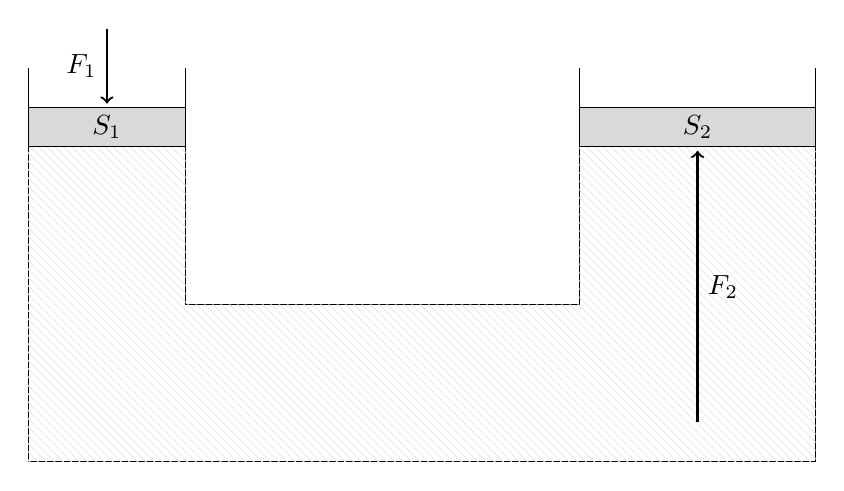
\begin{tikzpicture}
		% Draw the hydraulic container outline
		% \draw[thick] (0,0) -- (0,-4) -- (2,-4) -- (2,-1) -- (4,-1) -- (4,-4) -- (6,-4) -- (6,0);

		\draw (0,0) -- (0,-5) --(10,-5) -- (10,0)  (7,0) -- (7, -3) -- (2, -3) -- (2,0);

		\draw [draw = none, pattern = north west lines, pattern color=gray!15](0,-1) -- (0,-5) --(10,-5) -- (10,-1)  (7,-1) -- (7, -3) -- (2, -3) -- (2,-1);

		% Draw the left side piston (S1)
		\draw[ fill=gray!30] (0,-0.5) rectangle (2,-1);
		\node at (1,-0.75) {$S_1$};

		\draw[ fill=gray!30] (7,-0.5) rectangle (10,-1);
		\node at (8.5,-0.75) {$S_2$};
		% Draw the right side platform (S2)

		% Draw forces F1 and F2
		\draw[->, thick] (1,0.5) -- (1, -0.45) node[midway, left] {$F_1$};
		\draw[->, thick] (8.5,-4.5) -- (8.5,-1.05) node[midway, right] {$F_2$};


	\end{tikzpicture}
\end{center}
Secondo il principio di Pascal si ha che $ p_1  = p_2 $. Dato che $ p = \frac{F}{S} $, allora
\[
	\frac{F_1}{S_1} = \frac{F_2}{S_2}
\]
Questo significa che applicando una forza applicata sulla superficie piccola di un torchio idraulico risulterà più grande dall'altra parte del torchio, un po' in modo simile a ciò che accade con una leva

\subsection{Principio di archimede}
\begin{teorema}{Principio di Archimede}
	Il principio di Archimede enuncia che un corpo immerso in un liquido di densità $ \rho  $ subisce una spinta verso l'alto con intensità pari al peso di liquido spostato dalla parte immersa del corpo:
	\[
		F_a = \rho \cdot V_{\text{ immerso }} \cdot g
	\]
\end{teorema}
Nota che tramite la forza di archimede siamo in grado di capire se un corpo galleggia o meno:
\begin{center}
	\begin{tikzpicture}
		\draw (0,0)rectangle(2, -4);
		\draw (0,0)--(0,0.5);
		\draw (2,0)--(2,0.5);

		\coordinate (c) at (1,-1.5);
		\draw ($(c) + (-0.3,-0.3)$)rectangle($(c) + (0.3,0.3)$);
		\draw [thick, ->](c)--++(0,1) node[midway, right]{$ F_a $};
		\draw [thick, ->](c)--++(0,-1)node[midway, right]{$ P $};
		\node [whitedot] at (c){};
		\node ()[] at (1,-5) {$ P = F_a $};

		\begin{scope}[shift={(3,0)}]
			\draw (0,0)rectangle(2, -4);
			\draw (0,0)--(0,0.5);
			\draw (2,0)--(2,0.5);

			\coordinate (c) at (1,-0.2);
			\draw [fill=white]($(c) + (-0.3,-0.3)$)rectangle($(c) + (0.3,0.3)$);
			\draw [thick, ->](c)--++(0,1) node[midway, right]{$ F_a $};
			\draw [thick, ->](c)--++(0,-1)node[midway, right]{$ P $};
			\node [whitedot] at (c){};
			\node ()[] at (1,-5) {$ P < F_a $};
		\end{scope}

		\begin{scope}[shift={(6,0)}]
			\draw (0,0)rectangle(2, -4);
			\draw (0,0)--(0,0.5);
			\draw (2,0)--(2,0.5);

			\coordinate (c) at (1,-3.7);
			\draw ($(c) + (-0.3,-0.3)$)rectangle($(c) + (0.3,0.3)$);
			\draw [thick, ->](c)--++(0,1) node[midway, right]{$ F_a $};
			\draw [thick, ->](c)--++(0,-1)node[midway, right]{$ P $};
			\node [whitedot] at (c){};
			\node ()[] at (1,-5) {$ P > F_a $};
		\end{scope}
	\end{tikzpicture}
\end{center}

\section{Il moto}
In questa sezione sono descritti i principali strumenti e metodi per descrivere lo spostamento di un corpo nello spazio, bidimensionale e tridimensionale
\subsection{Definizioni}
Una serie di definizioni utili
\begin{definizione}{Traiettoria}
	La traiettoria di un corpo in movimento è la linea "tracciata" dal corpo in movimento al passare del tempo
\end{definizione}
\begin{definizione}{Moto rettilineo}
	Moto che avviene lungo una retta
\end{definizione}
\begin{definizione}{Intervallo di tempo}
	Un intervallo di tempo è la quantità di tempo trascorsa tra due istanti:
	\[
		\Delta t = t_2 - t_1
	\]
	dove $ t_2 $ è l'istante finale e $ t_1 $ è l'istante iniziale
\end{definizione}
\begin{definizione}{Spostamento}
	Lo spostamento è la differenza tra due posizioni
	\[
		\Delta s = s_2 - s_1
	\]
	dove $ s_2 $ è l'istante finale e $ s_1 $ è l'istante iniziale
\end{definizione}
Nota come la nozione di spostamento sia valida dal punto di vista logico sia in 1 che in 2 dimensioni:

% \begin{tikzpicture}
% 	\begin{axis}[
% 			xmin=0, xmax=5,
% 			ymin=0,ymax=5,
% 			restrict y to domain = 0:5, domain=0:5, width=0.98\textwidth, height=0.5\textwidth, grid=major, samples=200,  ylabel=$f(x)$, xlabel=$x$, legend entries={$ $}]
% 		\addplot[black, thick] {x};
% 	\end{axis}
% \end{tikzpicture}

% \begin{tikzpicture}
%   \draw (0,0)--(1,1);  
% \end{tikzpicture}

\begin{minipage}[c]{0.48\textwidth}
	\begin{tikzpicture}
		\draw [-latex](0,0)--(5,0);
		\node (s1)[whitedot, label={90:$ s_1 $}] at (1,0){};
		\node (s2)[whitedot, label={90:$ s_2 $}] at (4,0){};
		\draw [-latex](s1) to [bend left]  node [midway, above]{$ \Delta s $}(s2);
		\draw [red](s1)--(s2);
	\end{tikzpicture}
\end{minipage}
%
\begin{minipage}[c]{0.48\textwidth}
	\begin{tikzpicture}
		\begin{axis}[
				xmin=0, xmax=5,
				ymin=0,ymax=5,
				width=0.98\textwidth, height=0.98\textwidth, grid=major]
			\node (s1)[whitedot, label={$ s_1 $}] at (4,1){};
			\node (s2)[whitedot, label={$ s_2 $}] at (2,3){};
			\draw [-latex](0,0)--(s1);
			\draw [-latex](0,0)--(s2);
			\draw [-latex](s1)--(s2)node[midway, above right]{$ \Delta s $};
			\draw [red, -latex](s1)--(s2);
		\end{axis}
	\end{tikzpicture}
\end{minipage}
\subsection{La natura relativa del moto}
Poniamoci la seguente domanda:
\begin{center}
	\textit{Se ci trovassimo nella stiva di una nave completamente chiusa, riusciremmo a capire se siamo in movimento oppure no?}
\end{center}
La risposta è \underline{no}. Poniamoci dunque una domanda leggermente diversa:
\begin{center}
	\textit{Se ci trovassimo nella stiva di una nave, la quale sappiamo essere in moto, possiamo affermare di essere in moto?}
\end{center}
La risposta è \underline{dipende}. Questo perché il moto non è mai assoluto, bensì è sempre relativo a qualcos'altro, detto sistema di riferimento. Una risposta completa alla seconda domanda potrebbe dunque essere:
\begin{center}
	Siamo \textit{in moto rispettto al mare}, mentre siamo \textit{fermi rispetto alla nave}
\end{center}
Dunque quando parliamo di moto è sempre fondamentale fissare un sistema di riferimento, ossia "l'oggetto" rispetto al quale l'oggetto si sposta

\begin{definizione}{Sistema di riferimento cartesiano}
	Un sistema di riferimento cartesiano è il modo più comune per esprimere la posizione di un corpo. Questo è composto da due assi cartesiani i quali si intersecano in un punto detto \textit{origine}:
	\begin{tikzpicture}
		\begin{axis}[axis lines = center, xmin = 0, xmax = 4, ymin = 0, ymax = 4]
			\node [whitedot, label = {$ s_1 \left(2,2\right)$}] at (2,2){};
			\node [whitedot, label = {$ s_2 \left(3,3.5\right)$}] at (3,3.5){};
			\node [whitedot, label = {$ s_3 \left(1,1\right)$}] at (1,1){};
			\node [whitedot, label = {$ s_4 \left(3,1.5\right)$}] at (3,1.5){};
		\end{axis}
	\end{tikzpicture}
\end{definizione}
\subsection{Velocità e grafici}
\begin{definizione}{Velocità media}
	Per definizione la velocità media è data dallo spostamento per unità di tempo, dunque:
	\[
		V = \frac{\Delta x}{\Delta t} = \frac{s_2 - s_1}{t_2 - t_1}
	\]
	occhio che questa è la velocità media, quindi è possibile che il corpo si muova a velocità maggiori o minori negli istanti compresi tra $ t_1 $ e $ t_2 $
\end{definizione}
Spesso è utile rappresentare lo spostamento in funzione del tempo su di un grafico:
\begin{itemize}
	\item Asse $ x $: indica il tempo
	\item Asse $ y $: indica la posizione
\end{itemize}
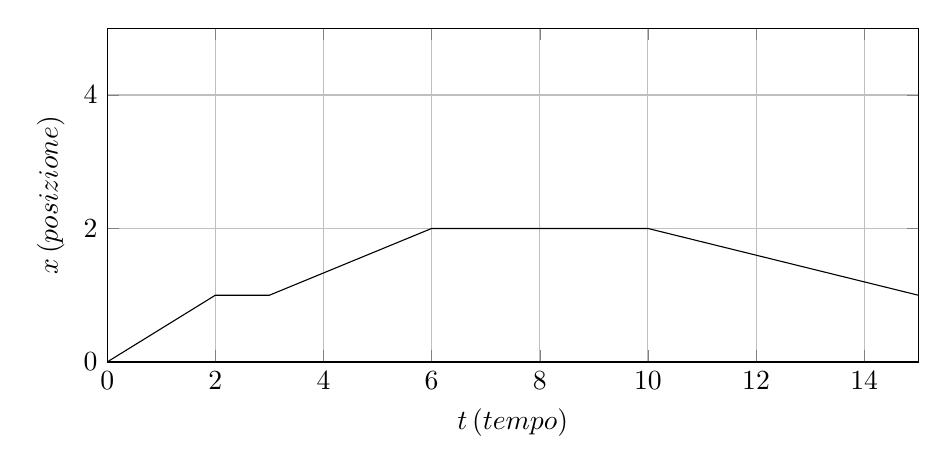
\begin{tikzpicture}
	\begin{axis}[
			xmin=0, xmax=15,
			ymin=0,ymax=5,
			restrict y to domain = 0:5, domain=0:5, width=0.98\textwidth, height=0.48\textwidth, grid=major, samples=200,  ylabel=$x \left(\text{posizione}\right)$, xlabel=$t \left(\text{tempo}\right)$]
		\draw (0,0)--(2,1)-- (3,1)--(6,2)-- (10,2)--(15, 1);
	\end{axis}
\end{tikzpicture}
Questo particolare grafico rappresenta la cosidetta \textit{legge oraraia} di un corpo
\begin{definizione}{Legge oraria}
	La legge oraria di un corpo non è altro che un'espressione matematica che esprime \textit{in funzione del tempo} la \textit{posizione} del suddetto corpo. Ad esempio:
	\[
		x\left(t\right) = 3 \cdot t
	\]
	è la legge oraria di un corpo che si sposta in avanti velocità costante
\end{definizione}
\subsection{Esercizi tipici MRU}
\begin{enumerate}
	\item Data lette oraria, rappresentala nel grafico spazio-tempo
	      \begin{itemize}
		      \item La legge oraria non è altro che una retta, quindi rappresentarla come si farebbe in matematica:
		            \[
			            s = v t + s_0
		            \]
		            corrisponde alla retta
		            \[
			            y = mx + q
		            \]
		            dove $ m = v $ e $ q = s_0 $
	      \end{itemize}
	\item Dato la rappresentazione del moto nel grafico spazio-tempo, ricavarne la legge oraria
	      \begin{itemize}
		      \item In questo caso bisogna ricavare il coefficiente angolare della retta e la sua quota. Il coefficiente angolare sarà la velocità, mentre la quota lo spostamento iniziale:
		            \[
			            m = v, \quad q = s_0
		            \]
		            ricordarsi che per ricavare $ m $ è sufficiente prendere due punti della retta e calcolare
		            \[
			            m = \frac{\Delta y}{\Delta x}  = \frac{y_1 - y_0}{x_1- x_0}
		            \]
	      \end{itemize}
	\item Data la legge oraria di due corpi, calcolare dove questi si incontrano:
	      \begin{itemize}
		      \item Date le leggi orarie:
		            \[
			            s_1 = v_1t + s_1  \quad  s_2 = v_2t + s_2
		            \]
		            per trovare il tempo al quali i corpi hanno la stessa posizione è sufficiente risolvere l'equazione di primo grado :
		            \[
			            v_1t + s_1 = v_2t + s_2
		            \]
		            per trovare poi la posizione in cui si incontrano, è sufficiente inserire il tempo trovato nell'equazione sopra in una delle due leggi orarie( è indifferente quale, in quanto i due corpi sono nella stessa posizione)
	      \end{itemize}
	\item Dedurre proprietà dei moti dal grafico, quali:
	      \begin{itemize}
		      \item Retta più ripida $ \rightarrow $ corpo più veloce
		      \item Retta piana $ \rightarrow  $ corpo fermo
		      \item Retta "in discesa" $ \rightarrow $ corpo va all'indietro
	      \end{itemize}
	\item Esercizi su scomposizione dei moti(es corpo che si muove in due dimensioni)
	      \begin{itemize}
		      \item In questo caso il moto va scomposto in due componenti, una su asse $ x $ e una su asse $ y $. Per far ciò è necessario ricordarsi delle regole della trigonometria indicate in sezione \ref{trigonometria}
	      \end{itemize}
\end{enumerate}
\subsection{Moto rettilineo uniformemente accelerato}
Introduciamo ora una nuova quantità fisica, ossia l'accelerazione. Intuitivamente l'accelerazione indica \underline{la velocità con cui la velocità stessa cambia}, ossia quanto rapidamente un corpo passa da una velocità $ v_1 $ ad una velocità $ v_2 $. Formalmente si indica con $ a $ ed è definita come segue:
\[
	a = \frac{\left(v_2 - v_1\right)}{t_2 - t_1} = \frac{\Delta v}{\Delta  t}
\]
nota che come nel caso della velocità questa formula esprima l'accelerazione \underline{media}.
\vskip3mm
\subsubsection{Legge oraria per moti accelerati}
Per esprimere la posizione di un corpo che accelera in funzione del tempo bisogna tenere conto dell'accelerazione nella legge oraria. In particolare, la legge oraria di un corpo che si muove di MRUA è:
\[
	x\left(t\right) = \frac{1}{2}at^2 + vt + x_0
\]
Quindi nel caso di moti accelerati ci toccherà operare con equazioni di secondo grado per via del $ t^2  $ che compare vicino allaccelerazione
\subsubsection{Grafici}
Osserviamo ora i seguenti grafici:
\vskip3mm
\begin{minipage}[t]{0.48\textwidth}
	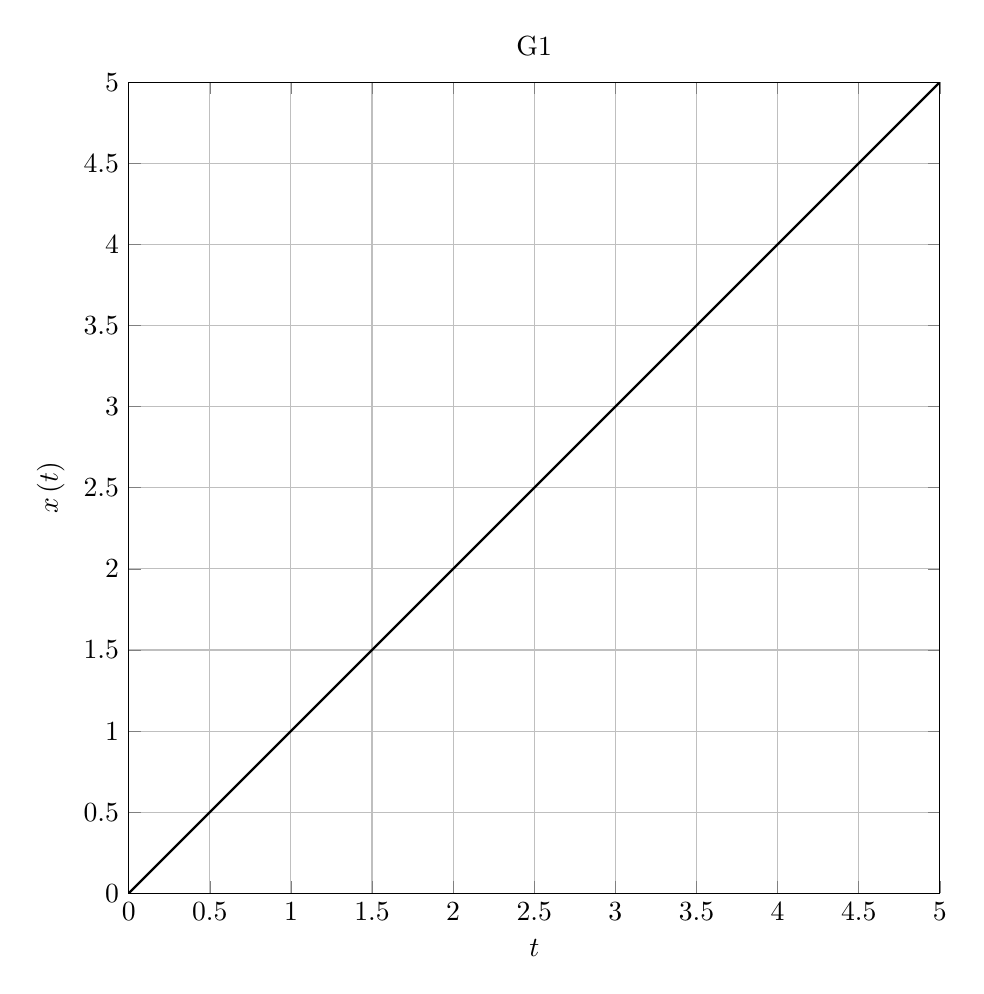
\begin{tikzpicture}
		\begin{axis}[
				xmin=0, xmax=5,
				ymin=0,ymax=5,
				restrict y to domain = 0:5, domain=0:5, width=0.98\textwidth, height=0.98\textwidth, grid=major, samples=200,  ylabel=$x\left(t\right)$, xlabel=$t$, title=G1]
			\addplot[black, thick] {x};
		\end{axis}
	\end{tikzpicture}
\end{minipage}
%
\begin{minipage}[t]{0.48\textwidth}
	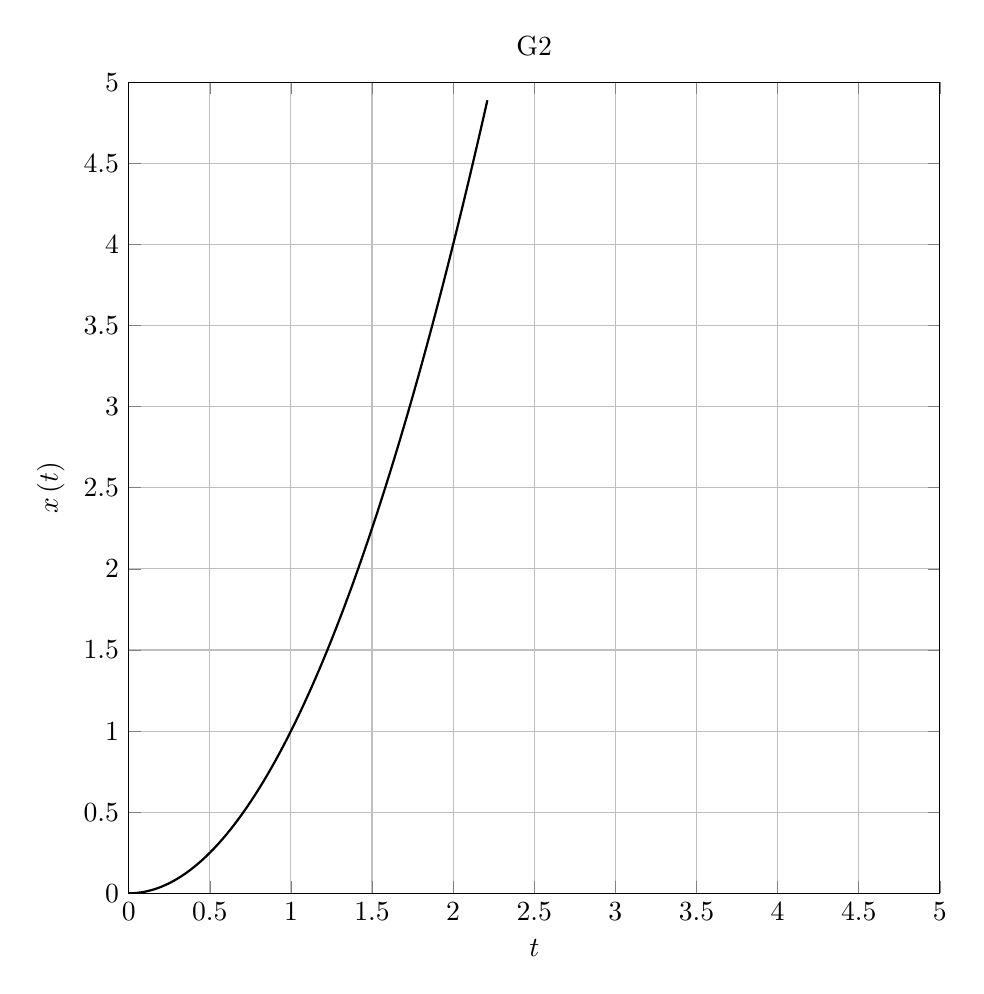
\begin{tikzpicture}
		\begin{axis}[
				xmin=0, xmax=5,
				ymin=0,ymax=5,
				restrict y to domain = 0:5, domain=0:5, width=0.98\textwidth, height=0.98\textwidth, grid=major, samples=200,  ylabel=$x\left(t\right)$, xlabel=$t$, title=G2]
			\addplot[black, thick] {x^2};
		\end{axis}
	\end{tikzpicture}
\end{minipage}
\vskip3mm
\begin{minipage}[t]{0.48\textwidth}
	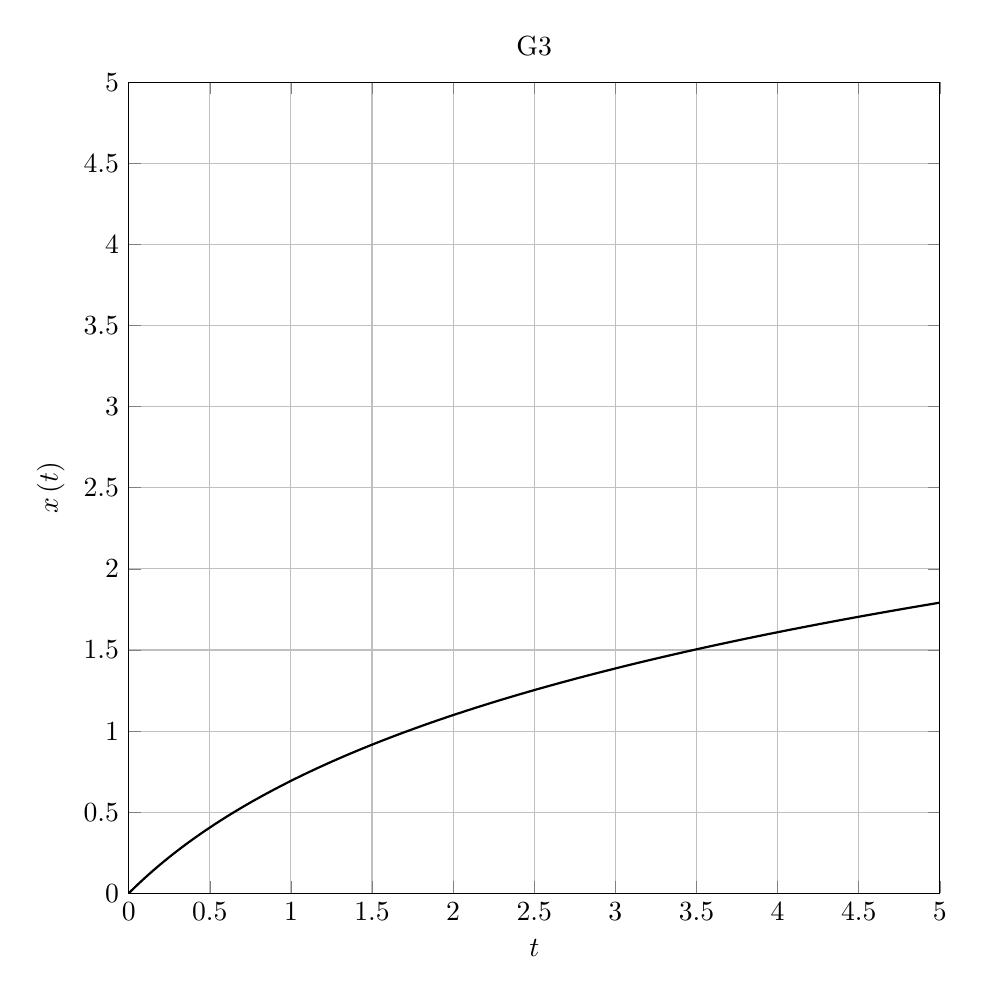
\begin{tikzpicture}
		\begin{axis}[
				xmin=0, xmax=5,
				ymin=0,ymax=5,
				restrict y to domain = 0:5, domain=0:5, width=0.98\textwidth, height=0.98\textwidth, grid=major, samples=200,  ylabel=$x\left(t\right)$, xlabel=$t$, title=G3]
			\addplot[black, thick] {ln(x+1)};
		\end{axis}
	\end{tikzpicture}
\end{minipage}
%
\begin{minipage}[t]{0.48\textwidth}
	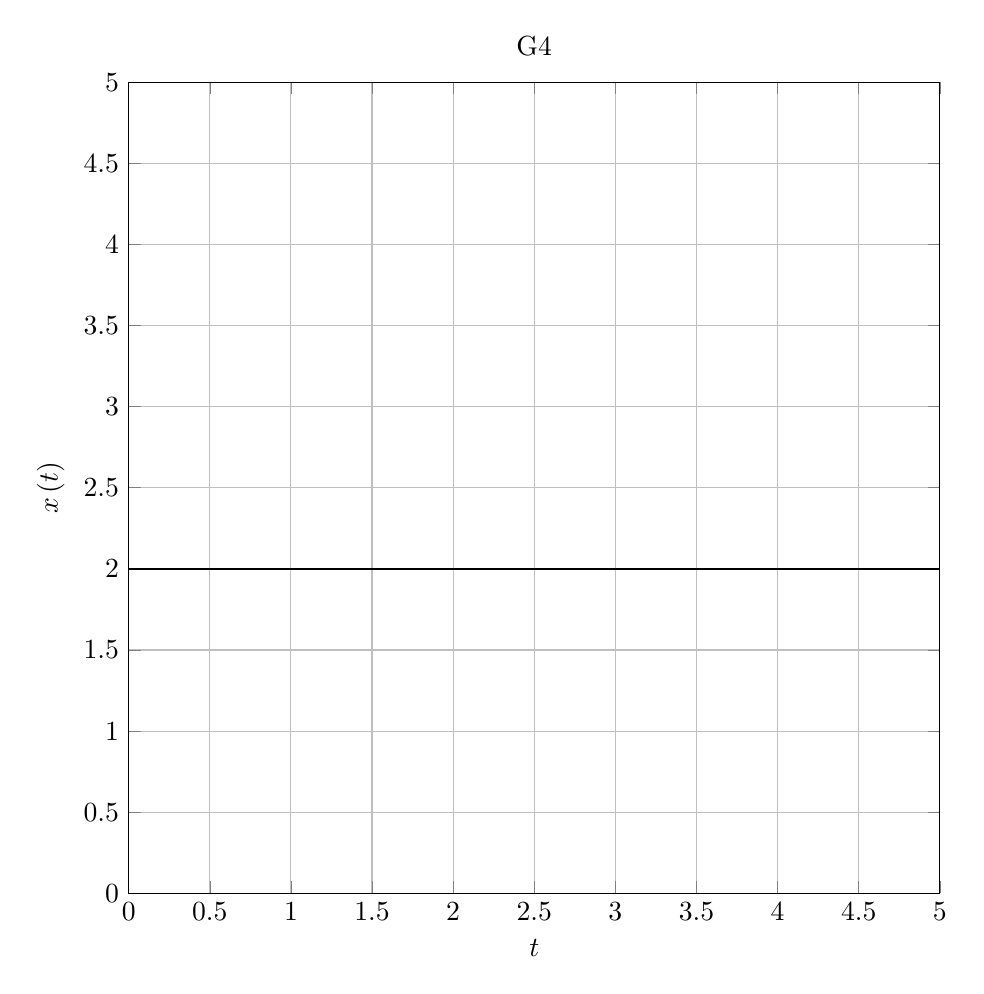
\begin{tikzpicture}
		\begin{axis}[
				xmin=0, xmax=5,
				ymin=0,ymax=5,
				restrict y to domain = 0:5, domain=0:5, width=0.98\textwidth, height=0.98\textwidth, grid=major, samples=200,  ylabel=$x\left(t\right)$, xlabel=$t$, title=G4]
			\addplot[black, thick] {2};
		\end{axis}
	\end{tikzpicture}
\end{minipage}
\vskip3mm
\begin{minipage}[t]{0.48\textwidth}
	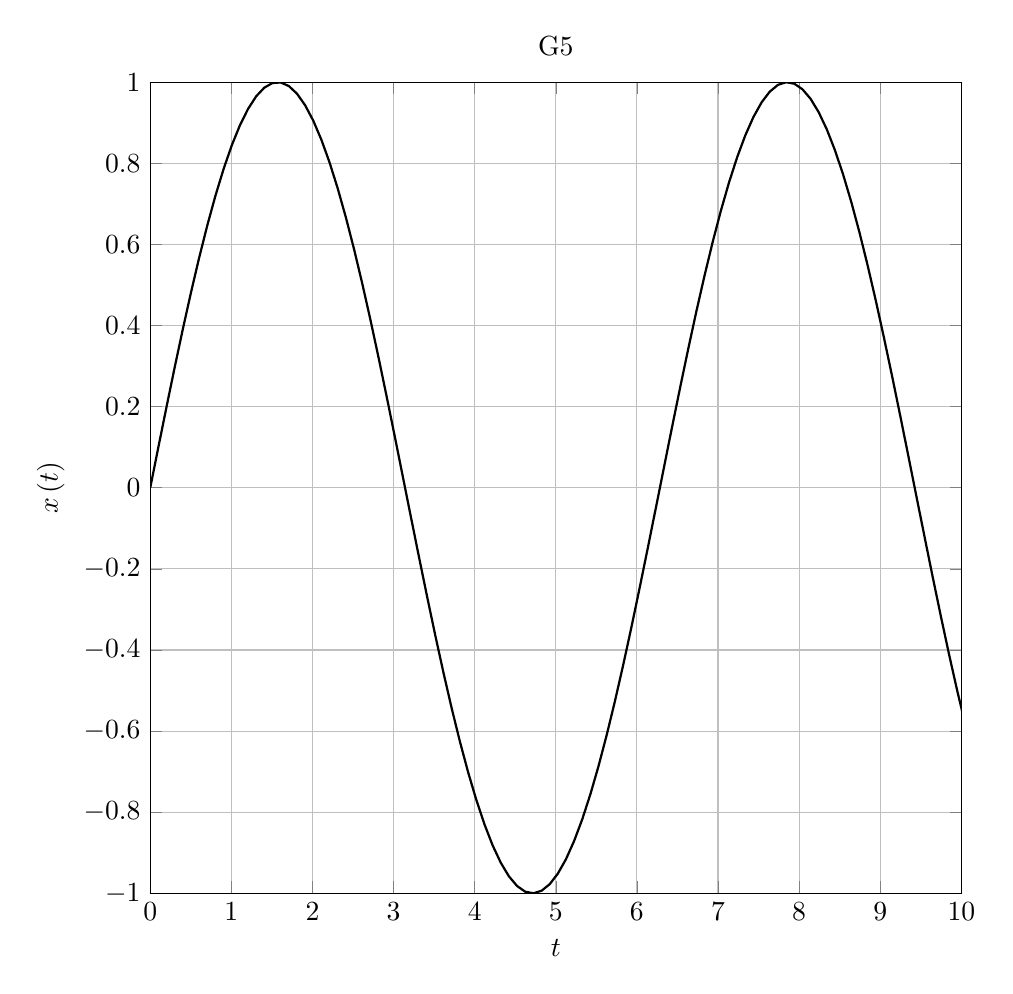
\begin{tikzpicture}
		\begin{axis}[
				xmin=0, xmax=10,
				ymin=-1,ymax=1,
				restrict y to domain = -1:1, domain=0:20, width=0.98\textwidth, height=0.98\textwidth, grid=major, samples=200,  ylabel=$x\left(t\right)$, xlabel=$t$, title=G5]
			\addplot[black, thick] {sin(deg(x))};
		\end{axis}
	\end{tikzpicture}
\end{minipage}
%
\begin{minipage}[t]{0.48\textwidth}
	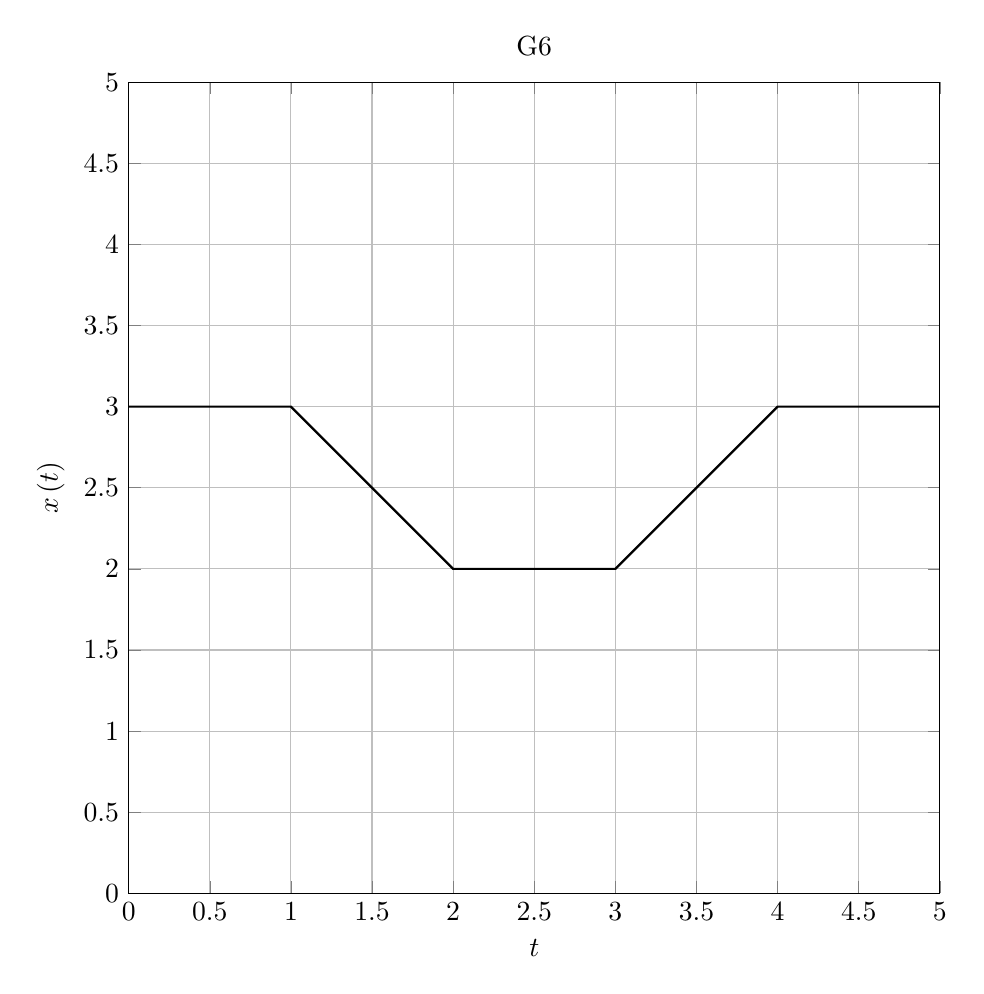
\begin{tikzpicture}
		\begin{axis}[
				xmin=0, xmax=5,
				ymin=0,ymax=5,
				restrict y to domain = 0:5, domain=0:5, width=0.98\textwidth, height=0.98\textwidth, grid=major, samples=200,  ylabel=$x\left(t\right)$, xlabel=$t$, title=G6]
			\draw [thick](0,3)--(1,3)--(2,2)--(3,2)--(4,3)--(5,3);
		\end{axis}
	\end{tikzpicture}
\end{minipage}
\vskip3mm
Quali dei seguenti grafici possono essere relativi a moti rettilinei uniformemente accelerati?  (Ricordarsi che la velocità è la pendenza della tangente al grafico)
\begin{enumerate}
	\item G1 e G2 non possono esserlo in quanto la tangente ha sempre la stessa inclinazione, dunque la velocità è sempre la stessa
	\item G2, G3, G5 sono accelerati in quanto la pendenza della tangente al grafico cambia, dunque la velocità cambia per via di una accelerazione
	\item G6 rappresenta una situazione un po' particolare. Nei tratti $ \left[0,1\right], \left[1,2\right], \left[2,3\right],\left[3,4\right], \left[4,5\right] $ il moto di muove di MRU. Il problema sta nel capire cosa accade nei punti angolosi. Disegnamo il grafico $ v\left(t\right), t $ per capire meglio
\end{enumerate}
\vskip3mm
\begin{minipage}[c]{0.48\textwidth}
	\begin{tikzpicture}
		\begin{axis}[
				xmin=0, xmax=5,
				ymin=-2,ymax=2,
				restrict y to domain = -5:5, domain=0:5, width=0.98\textwidth, height=0.98\textwidth, grid=major, samples=200,  ylabel=$v\left(t\right)$, xlabel=$t$, title=G6]
			\draw [thick](0,0)--(1,0);
			\draw [thick](1,-1)--(2,-1);
			\draw [thick](2,0)--(3,0);
			\draw [thick](3,1)--(4,1);
			\draw [thick](4,0)--(5,0);

			\node (1)[whitedot] at (1,0){};
			\node (2)[blackdot] at (1,-1){};

			\node (3)[blackdot] at (2,0){};
			\node (4)[whitedot] at (2,-1){};

			\node (5)[whitedot] at (3,0){};
			\node (6)[blackdot] at (3,1){};

			\node (7)[blackdot] at (4,0){};
			\node (8)[whitedot] at (4,1){};

			\node (p1)[anchor=east] at (1,-0.5)  {$ p_1 $};
			\node (p2)[anchor=west] at (2,-0.5)  {$ p_2 $};
			\node (p3)[anchor=east] at (3,0.5)  {$ p_3 $};
			\node (p4)[anchor=west] at (4,0.5)  {$ p_4 $};

			\draw [dotted](p1)edge(1)edge(2);
			\draw [dotted](p2)edge(3)edge(4);
			\draw [dotted](p3)edge(5)edge(6);
			\draw [dotted](p4)edge(7)edge(8);

		\end{axis}
	\end{tikzpicture}
\end{minipage}
%
\begin{minipage}[c]{0.48\textwidth}
	Nei punti $ p_1, p_2,p_3, p_4 $ effettivamente la velocità cambia, ma istantaneamente. Ciò nella vita reale è impossibile, ma in un modello può aver senso. Rimane il problem che calcolando l'accelerazione in ognuno di questi punti si avrebbe:
	\[
		a = \frac{\Delta v}{\Delta t} = \frac{1}{0} \rightarrow \text{ \underline{impossibile} }
	\]
\end{minipage}
\subsubsection{Grafico velocità tempo}
Come possiamo relazionare lo spostamento al tempo nel grafico $ x- t $, possiamo anche relazionare l'andamento della velocità nel tempo tramite un grafico $ v- t $. In maniera del tutto analoga al grafico $ v- t $, possiamo affermare le seguenti cose:
\begin{enumerate}
	\item L'inclinazione della retta tangente al grafico in un punto $ p $ costituisce \underline{l'accelerazione} in quel punto
	\item Il grafico $ v- t$ di un MRU sarà dato da una linea "piatta", con equazione $ t=v $
\end{enumerate}

\subsubsection{Grafico accelerazione tempo}
Questo grafico è molto meno interessante in quanto ci limitiamo ad analizzare moti con accelerazione costante. Il grafico sarà dunque costituito da una semprile linea piatta orizzontale, con equazione $ y = a $
\subsubsection{Conversione grafici}
Per passare da un tipo di grafico all'altro possiamo seguire il seguente schema:
\vskip3mm
\begin{center}
	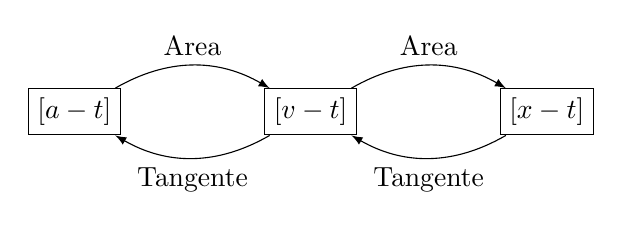
\begin{tikzpicture}
		\node (1)at (-3, 0)[draw]  {$\left[a-t\right] $};
		\node (2)at(0, 0)[draw]  {$ \left[v - t\right] $};
		\node (3)at(3, 0)[draw]  {$ \left[x-t\right] $};
		\draw [-latex](1)to[bend left]node [midway, anchor = south]{Area}(2);
		\draw [-latex](2)to[bend left]node [midway, anchor = south]{Area}(3);
		\draw [-latex](3)to[bend left]node [midway, anchor = north]{Tangente}(2);
		\draw [-latex](2)to[bend left]node [midway, anchor = north]{Tangente}(1);
	\end{tikzpicture}
\end{center}
In particolare il metodo dell'area e della tangente si comportano come segue:
\begin{enumerate}
	\item AREA: il grafico calcolato in $ p $ vale quanto la somma dell'area sottesa al grafico di partenza fino a $ p $. Nota che l'area va intesa con il segno, come in figura \ref{areaconsegno}
	\item TANGENTE: il grafico calcolato in $ p $ vale quanto l'inclinazione della retta tangente in $ p $ nel grafico di partenza
\end{enumerate}
\usepgfplotslibrary{fillbetween}
\begin{figure}
	\label{areaconsegno}
	\begin{tikzpicture}
		\begin{axis}[
				xmin=0, xmax=4*pi,
				ymin=-2,ymax=2,
				restrict y to domain = -2:2, domain=0:15, width=0.98\textwidth, height=0.5\textwidth, grid=major, samples=200,  ylabel=$f(x)$, xlabel=$x$]
			\addplot[black, thick, name path=A] {sin(deg(x))};
			\addplot[draw=none,name path=B] {0};
			\addplot[green!20, opacity=0.5] fill between[of=A and B,soft clip={domain=0:pi}];
			\addplot[green!20, opacity=0.5] fill between[of=A and B,soft clip={domain=2*pi:3*pi}];
			\addplot[red!20, opacity=0.5] fill between[of=A and B,soft clip={domain=pi:2*pi}];
			\addplot[red!20, opacity=0.5] fill between[of=A and B,soft clip={domain=3*pi:4*pi}];
			\draw (0,0)--(4 * pi, 0);
		\end{axis}
	\end{tikzpicture}
	\caption{Segno area sottesa al grafico}
\end{figure}



\section{Equazioni di secondo grado e parabole}

\subsection{Terminologia}
\begin{definizione}{Forma normale}
	Un'equazione si dice in forma normale se è scritta come un'equzione tra un polinomio e zero e non si può semplificare nulla
\end{definizione}
\begin{itemize}
	\item Equazioni in forma normale:
	      \begin{align*}
		      15x^{4} + x^2  -2x + 2 = 0 &  & 12x = 0 &  & x^2 + 1 = 0
	      \end{align*}
	\item Equazioni che \underline{NON} sono in forma normale:
	      \begin{align*}
		       & 12x = 1 &  & x^2 - x^2  +x = 0
	      \end{align*}
\end{itemize}
non lo sono.

\begin{definizione}{Equazione di secondo grado}
	Un'equazione si dice di secondo grado se, una volta ridotta in forma normale l'esponente di grado massimo è uguale a 2
\end{definizione}
\begin{itemize}
	\item Equazioni di secondo grado:
	      \begin{align*}
		       & 5x^2 -2x + 1 = 0 &  & 5x^2 -2x + 1 = 2x^2  -2 \\
		       & x^2  = -1        &  & x^2 -2x = 0
	      \end{align*}
	\item Equazioni che \underline{NON} sono di secondo grado:
	      \begin{align*}
		       & 2x + 1 = 0     &  & 5x^2 -5x^2  + 1 =  -2 \\
		       & x^2  = x^2 + x &  & 3x + 2 = -2x
	      \end{align*}
\end{itemize}

\begin{definizione}{Equazioni complete, pure, spurie, monomi}
	Un' equazione di \underline{secondo grado} può essere classificata in base a quali suoi coefficienti valgono. Una generica equazione di secondo grado
	\[
		ax^2  + bx + c = 0
	\]
	viene detta:
	\begin{itemize}
		\item \textit{Completa} se ne $ a $ ne $ b $ ne $ c $ valgono 0: $ 15x^2  + 2x -10 = 0  $
		\item \textit{Pura} se solo $ b = 0 $: $ 15x^2  - 10 = 0 $
		\item \textit{Spuria} se solo $ c = 0 $: $ 15x^2 +2x = 0  $
		\item \textit{Monomia} se sia $ b $ che $ c $ valgono 0: $ 15x^2 = 0 $
	\end{itemize}
\end{definizione}\label{tipiequazionisecondogrado}

\subsection{Risoluzione equazioni di secondo grado}
Ci occupiamo intanto della risoluzione delle equazioni \underline{NON} fratte. Lo schema risolutivo è il seguente:
\begin{enumerate}
	\item Tramite le proprietà delle equazioni, riduco al l'equazione nella sua \underline{forma normale}
	\item Trovare i risultati come indicato qui sotto, in base al tipo della equazione ottenuta vedi definizione \ref{tipiequazionisecondogrado}
\end{enumerate}
\subsubsection{Equazioni complete}
Per questo tipo di equazione esiste una formula nella quale possiamo inserire i parametri per ricavare le soluzioni. Data un'equazione di secondo grado nella seguente forma:
\[
	ax^2  + bx + c = 0
\]
allora le soluzioni sono date da
\[
	x_{1/2} = \frac{-b \pm \sqrt{b^2  - 4 ac}}{2a}
\]
nota che
\begin{itemize}
	\item La quantità $ \sqrt{b^2  - 4ac} $ è detta \underline{determinante} e si indica con $ \Delta  $
	\item Questa formula può produrre 0,1 o 2 soluzioni a seconda del valore di $ \Delta  $:
	      \begin{itemize}
		      \item $ \Delta < 0 $: 0 soluzioni
		      \item $ \Delta = 0 $: 1 soluzione
		      \item $ \Delta > 0 $: 2 soluzioni
	      \end{itemize}
\end{itemize}
\subsubsection{Esempio}
Supponendo di avere:
\[
	2x^2  - 4x - 6
\]
le soluzioni sono date da
\begin{center}
	\begin{tikzpicture}
		\node (formula)[] at (0,0) {$ \displaystyle x_{1/2} = \frac{4 \pm \sqrt{\left(-4\right)^2  - 4 (2) \cdot (-6)}}{2 \cdot 2} = \frac{4 \pm \sqrt{64}}{4} = \frac{4 \pm 8}{4}$};
		\node (solution1)[above right = -0.5em and 2em of formula] {$ \displaystyle x_1 = \frac{12}{4} = 3 $};
		\node (solution2)[below right = -0.5em and 2em of formula]  {$ \displaystyle x_2 = \frac{-4}{4} = -1 $};
		\draw [->] (formula.east) to [out=0, in=180] (solution1.west);
		\draw [->] (formula.east) to [out=0, in=180] (solution2.west);
	\end{tikzpicture}
\end{center}

\subsubsection{Equazioni pure}
Per questo tipo di equazioni è sufficiente portare a destra $ a $ e $ c $ ed eseguire la radice da entrambe le parti. Occhio al "$ \pm $"!
\[
	ax^2 + c  = 0 \rightarrow ax^2  = -c \rightarrow x^2  = \frac{-c}{a} \rightarrow x = \pm \sqrt{\frac{-c}{a}}
\]
Nota che
\begin{itemize}
	\item Nell'ultimo passaggio va messo sempre il $ \pm $. Basti pensare a $ x^2  = 4 $. Chiaramente $ 2 \cdot 2 = 4 $ ma anche $ -2 \cdot  -2  = 4$. Questo è vero per \underline{qualsiasi numbero}!
	\item Le equazioni pure hanno sempre 2 o 0 soluzioni, nel caso alla destra io ottenga rispettivamente un numero positivo o negativo
\end{itemize}
\subsubsection{Esempio}
Supponendo di avere:
\[
	4x^2 -9 = 0
\]
allora procedo così:
\[
	4x^2 = 9 \rightarrow \sqrt{4x^2 } = \sqrt{9} \rightarrow 2x = 3 \rightarrow x = \frac{3}{2}
\]

\subsubsection{Equazioni spurie}
Per questo tipo di equazioni si può sempre effettuare un raccoglimento della $ x $, applicando poi la legge dell'annullamento del prodotto:
\begin{center}
	\begin{tikzpicture}
		\node (formula)[] at (0,0) {$ \displaystyle ax^2  + bx = 0 \rightarrow x\left(ax + b\right) = 0 $};
		\node (solution1)[above right = -0.5em and 2em of formula] {$ \displaystyle x_1 = 0 $};
		\node (solution2)[below right = -0.5em and 2em of formula]  {$ \displaystyle x_2 = \frac{-b}{a} $};
		\draw [->] (formula.east) to [out=0, in=180] (solution1.west);
		\draw [->] (formula.east) to [out=0, in=180] (solution2.west);
	\end{tikzpicture}
\end{center}

Nota che:
\begin{itemize}
	\item Ho sempre esattamente 2 soluzioni
	\item Una soluzione è sempre 0. Questo perché la $ x $ compare in ogni fattore. Quando questa si annulla, l'equazione sarà sempre soddisfatta
\end{itemize}

\subsubsection{Esempio}
Supponiamo di avere:
\[
	5x^2  - 2x = 0
\]
allora risolvo così
\begin{center}
	\begin{tikzpicture}
		\node (formula)[] at (0,0) {$ \displaystyle 5x^2 -2x = 0 \rightarrow x\left(5x - 2\right) = 0 $};
		\node (solution1)[above right = -0.5em and 2em of formula] {$ \displaystyle x_1 = 0 $};
		\node (solution2)[below right = -0.5em and 2em of formula]  {$ \displaystyle \left(5x-2\right) = 0 \rightarrow x_2 = \frac{5}{2} $};
		\draw [->] (formula.east) to [out=0, in=180] (solution1.west);
		\draw [->] (formula.east) to [out=0, in=180] (solution2.west);
	\end{tikzpicture}
\end{center}

\subsubsection{Monomie}
Il caso delle equazioni monomie è particolarmente semplice. La soluzione è \underline{una}, ossia 0
\[
	ax^2 = 0 \rightarrow x = 0
\]

\subsection{Grafico di una parabola}
Per disegnare una parabola sul piano cartesiano possono esserci utilile seguenti nozioni. Consideriamo
\[
	y = ax^2  + bx + c
\]
\begin{itemize}
	\item Se $ a < 0 $ allora la parabola ha concavità verso il basso, altrimenti verso l'alto
	      \begin{minipage}[t]{0.48\textwidth}
		      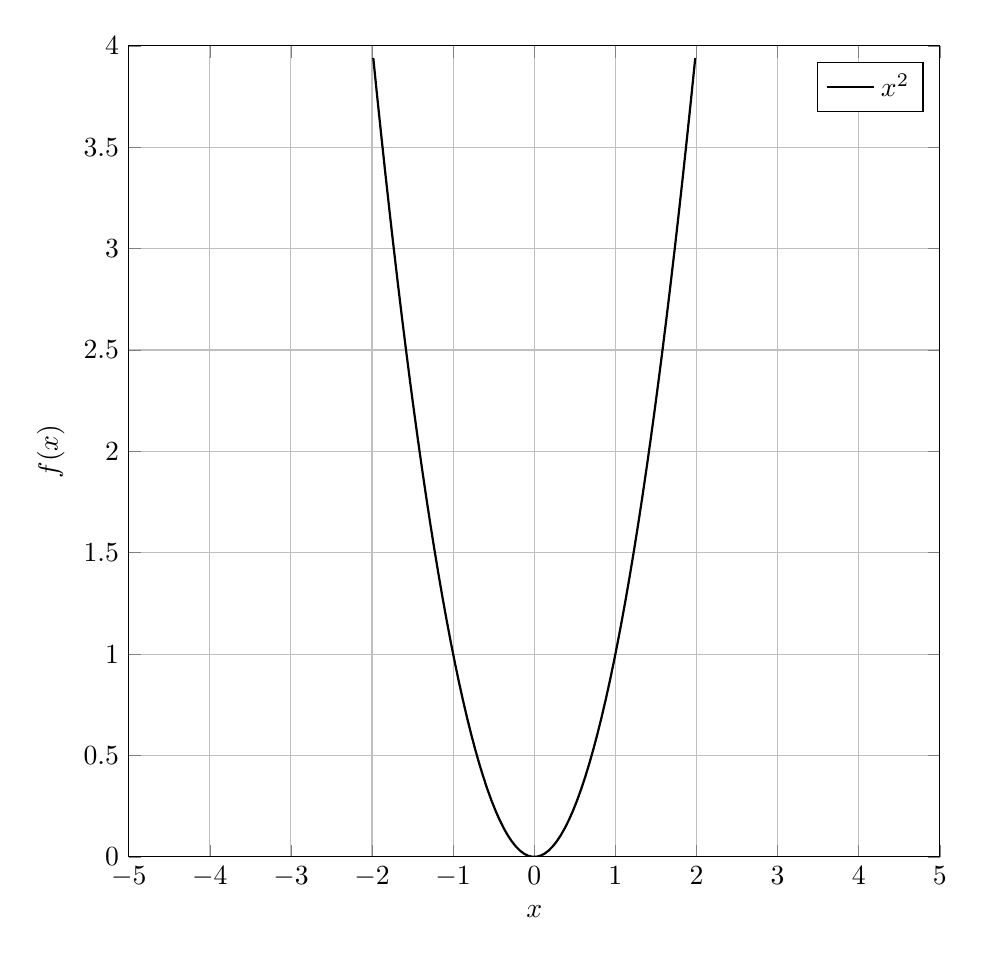
\begin{tikzpicture}
			      \begin{axis}[
					      xmin=-5, xmax=5,
					      ymin=0,ymax=4,
					      restrict y to domain = -4:4, domain=-5:5, width=0.98\textwidth, height=0.98\textwidth, grid=major, samples=200,  ylabel=$f(x)$, xlabel=$x$, legend entries={$ x^2 $}]
				      \addplot[black, thick] {x^2};
			      \end{axis}
		      \end{tikzpicture}
	      \end{minipage}
	      %
	      \begin{minipage}[t]{0.48\textwidth}
		      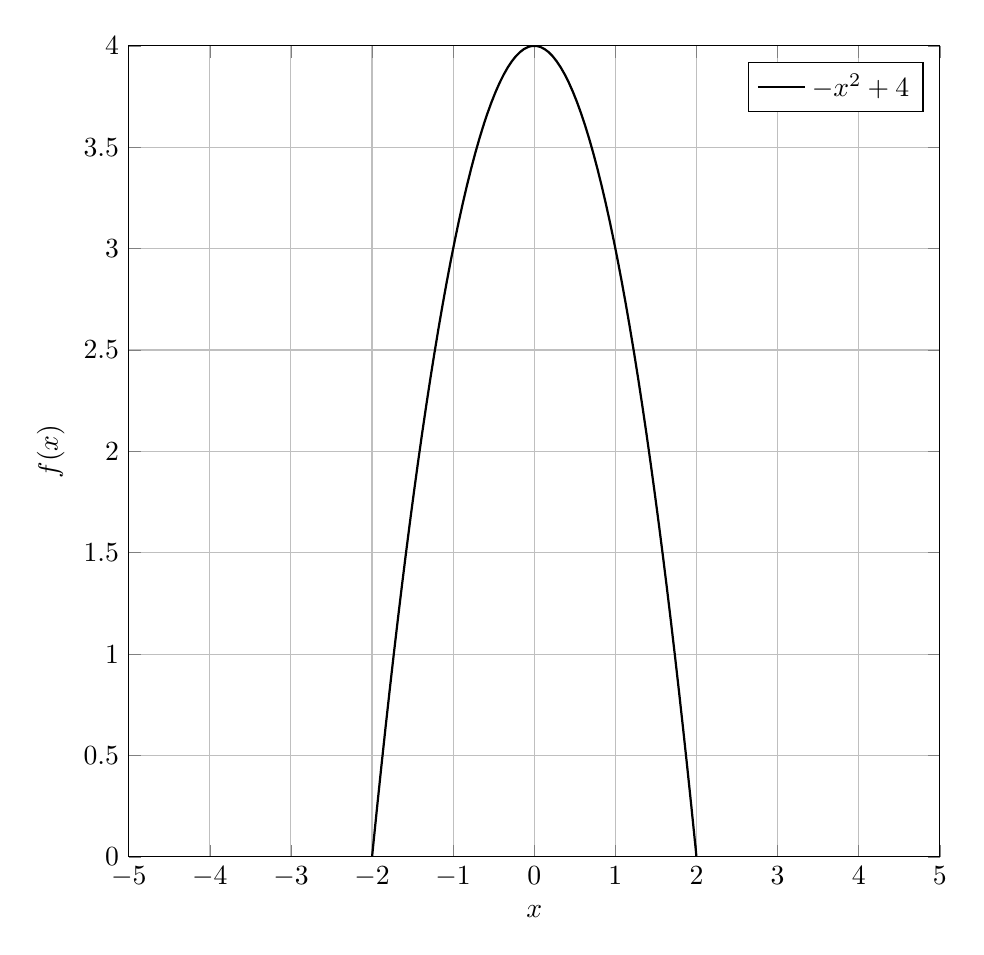
\begin{tikzpicture}
			      \begin{axis}[
					      xmin=-5, xmax=5,
					      ymin=0,ymax=4,
					      restrict y to domain = -4:4, domain=-5:5, width=0.98\textwidth, height=0.98\textwidth, grid=major, samples=200,  ylabel=$f(x)$, xlabel=$x$, legend entries={$ -x^2  + 4$}]
				      \addplot[black, thick] {-x^2 + 4};
			      \end{axis}
		      \end{tikzpicture}
	      \end{minipage}
	\item Il vertice ha coordinate
	      \[
		      \left(\frac{-b}{2a}, \frac{-\Delta }{4a}\right)
	      \]
	\item La parabola incontra l'asse x nelle x che risolvono l'equazione associata (ossia quella ottenuta ponendo la funzione = 0)
	\item Il valore $ c $ è detto \textit{quota}, e indica il punto in cui la parabola incrocia l'asse $ y $
	\item Il coefficiente $ a $, indica quanto "ripida è la parabola"
	      \begin{center}
		      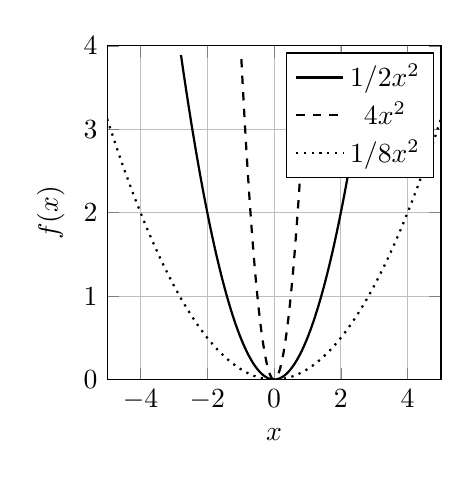
\begin{tikzpicture}
			      \begin{axis}[
					      xmin=-5, xmax=5,
					      ymin=0,ymax=4,
					      restrict y to domain = -4:4, domain=-5:5, width=0.48\textwidth, height=0.48\textwidth, grid=major, samples=200,  ylabel=$f(x)$, xlabel=$x$, legend entries={$ 1/2x^2 $, $4x^2$, $ 1/8 x^2  $}]
				      \addplot[black, thick] {1/2*x^2};
				      \addplot[dashed, thick] {4*x^2};
				      \addplot[dotted, thick] {1/8*x^2};
			      \end{axis}
		      \end{tikzpicture}
	      \end{center}
\end{itemize}

\section{Termodinamica}
\subsection{Dilatazione termica}
\begin{definizione}{Dilatazione termica lineare}
	Dato un oggetto di lunghezza $ L_0 $ e un cambiamento di temperatura di $ \Delta T $ gradi, allora la dilatazione lineare è pari a
	\[
		\Delta L = L_0 \cdot \gamma \cdot \Delta T
	\]
	dove $ \gamma $ è il coefficiente di dilatazione lineare, che è una costante caratteristica del materiale.
\end{definizione}
\begin{definizione}{Dilatazione termina superficiale}
	Dato un oggetto di area $ A_0 $ e un cambiamento di temperatura di $ \Delta T $ gradi, allora la dilatazione quadratica è pari a
	\[
		\Delta A = A_0 \cdot \gamma \cdot \Delta T
	\]
	dove $ \gamma $ è il coefficiente di dilatazione quadratica, che è una costante caratteristica del materiale.
\end{definizione}
\begin{definizione}{Dilatazione termica volumetrica}
	Dato un oggetto di volume $ V_0 $ e un cambiamento di temperatura di $ \Delta T $ gradi, allora la dilatazione cubica è pari a
	\[
		\Delta V = V_0 \cdot \gamma \cdot \Delta T
	\]
	dove $ \gamma $ è il coefficiente di dilatazione cubica, che è una costante caratteristica del materiale.
\end{definizione}

\begin{teorema}{Rapporto tra coeffienti di dilatazione termica}
	I coefficienti di dilatazione termica lineare($ \gamma $), superficiale $ \gamma_2 $ e volumetrica $ \gamma_3 $ sono legati dalla relazione:
	\begin{align*}
		\gamma_3 & = 3 \cdot \gamma \\
		\gamma_2 & = 2 \cdot \gamma
	\end{align*}
\end{teorema}

\subsection{Calore}
Il calore è una forma di energia che è presente nel momento in cui due corpi di scambiano, per l'appunto, \textit{calore}
\begin{definizione}{Calore specifico}
	Il calore specifico è la quantità di calore necessaria per aumentare la temperatura di un grammo di sostanza di un grado Celsius.
	\[
		Q = c \cdot m \cdot \Delta T
	\]
\end{definizione}
quando di usano quete formule è necessario ricordarsi di usare i gradi Kelvin:
\[
	\text{ gradi Kelvin } = \text{ gradi Celsius } + 273
\]
inoltre è spesso utile la caloria come unità di misura del calore:
\[
	1 \operatorname{[cal]} = 4.1868 \operatorname{[J]}
\]
\section{Riassuntone}
\subsection{Equazioni e disequazoni}
Equazioni e disequazioni sono la base di ogni argomento che tratterai, quindi è importante averci familiarità.
\subsubsection{Equazioni}
Per risolvere le equazioni la stratega di base è sempre la stessa:
\begin{itemize}
	\item Fare le C.E.
	\item Portare tutto a sinistra
	\item Mettere tutto a comune denominatore
	\item Imporre il numeratore = 0
	\item Verificare che le soluzioni trovate non appartengano ai valori esclusi dalle C.E.
\end{itemize}
\textit{Imporre} il numeratore = 0 significa rsolvere un'equazone di grado $ x $. Questo, in base al caso, può voler dire:
\begin{itemize}
	\item Risolvere un' equazione di primo grado, in questo modo:
	      $ ax + b = 0 \rightarrow ax = b \rightarrow x = \frac{b}{a} $
	\item Risolvere un'equazione di secondo grado, il che può essere fatto iin pui modi:
	      \begin{itemize}
		      \item Scomposizioine tramite trinomio speciale
		      \item Applicando la formula risolutiva:
		            \[
			            x_{1/2} = \frac{-b \pm \sqrt{b^2 - 4ac}}{2a}
		            \]
	      \end{itemize}
	\item Risolvere un'equazione di grado superiore al secondo, il che può richiedere "un po' di fantasia". Di solito si ricorre alla scomposizione tramite prodotti notevoli e raccoglimenti
\end{itemize}

\subsubsection{Disequazioni}
Il procedimento per risolvere una disequazione è uguale a quello per risolvere l'equazione associata, tuttavia vi è una differenza nell'ultimo step. In particolare, una volta ottenuta una forma del tipo:
\[
	\frac{A}{B} \ge 0
\]
è necessario sudiare il segno di numerattore e denominatore separatamente.

\subsection{Rette}
Una retta è definita da un'equazione nella forma:
\[
	y = mx + q
\]
dove $ m $ è detto \textit{coefficiente angolare} e  $ q $ è detta \textit{quota}. In particolare:
\begin{itemize}
	\item $ m $ indica di quanto "sale" sulla $ y $ ogni spostamento di 1 sulla x. Nello specifico, per ogni punto che appartenga alla retta vale:
	      \[
		      m = \frac{\Delta y}{\Delta x}
	      \]
	\item $ q $ definisce l'altezza del punto di inersezione fra la retta e l'asse $ y $
\end{itemize}
\subsection{Parabola}
Una parabola è definita da un'equazione nella forma:
\[
	y = ax^2 + bx + c
\]
\begin{itemize}
	\item Se $ a > 0 $ la parabola ha concavità verso l'alto, altrimenti verso il basso
	\item Quanto più grande è $ \left|a\right| $ tanto più "ripida" è la parabola
	\item $ c $ definisce l'altezza del punto di intersezione fra la parabola e l'asse $ y $
\end{itemize}
In più, il vertice della parabola ha coordinate:
\[
	\left(\frac{-b}{2a}, \frac{-\Delta }{4a}\right)
\]

\section{Moto armonico e moto circolare uniforme}
Innanzitutto, per affrontare questo argomenti è necessario avere una base matematica per quanto riguarda le funzioni goniometriche. In particolare, è necessario sapere lavorare bene con seni e coseni e tangenti.
\subsection{Funzioni goniometriche}
Inanzittuto il signifcato geometrico seno, coseno e tangente è il seguente. Data una circonferenza di raggio 1, e dato un punto su di essa che forma un angolo $ \theta $ con l'asse $ x $ , allora abbiamo che:
\begin{itemize}
	\item $ \sin \left(\theta \right) $ è la lunghezza della proiezione sull'asse $ y $ del punto
	\item $ \cos  \left(\theta \right) $ è la lunghezza della proiezione sull'asse $ x $ del punto
	\item $ \tan \left(\theta \right) $ è la lunghezza della retta che parte dall'origine e tocca la retta tangente alla circonferenza nel punto $ \left(1,0\right) $
\end{itemize}

\begin{tikzpicture}
	\begin{axis}[
			xmin=-1.5, xmax=1.5,
			ymin=-1.5, ymax=1.5,
			restrict y to domain = -1:1, domain=-1:1, width=0.7\textwidth, height=0.7\textwidth, grid=major, samples=200,  ylabel=$y$, xlabel=$x$]
		\draw[thick] (0,0) circle [radius=1];
		\draw[thick] (0.2,0) arc[start angle=0,end angle=30,radius=0.2];
		\node [anchor = south] at (0.3,0) {$\theta$};
		\draw [thick](0,0)--(30:1);
		\coordinate (cosc) at ($(0,0)!(30:1)!(1,0)$);
		\coordinate (sinc) at ($(0,0)!(30:1)!(0,1)$);
		\draw [dotted](0,0)--(1,{tan(30)});
		\draw [dotted](30:1)--(cosc);
		\draw [dotted](30:1)--(sinc);
		\draw (0,0)--(1,0);
		\draw (0,0)--(0,1);


		\begin{scope}[xshift=-0.1cm]
			\draw [latex-latex, dashed] (0,0) -- ($(0,0)!(30:1)!(0,1)$) node[midway, left] {$\sin(\theta)$};
		\end{scope}
		\begin{scope}[xshift=0.1cm]
			\draw [latex-latex, dashed] (1,0) -- (1,{tan(30)}) node[midway, right] {$\tan (\theta)$};
		\end{scope}
		\begin{scope}[yshift=-0.1cm]
			\draw [latex-latex, dashed] (0,0) -- ($(0,0)!(30:1)!(1,0)$) node[midway, below] {$\cos (\theta)$};
		\end{scope}

		% \draw [<->, draw=mutedblue](0,0)--(cosc) node[midway, below] {$ \cos\left(\theta\right)$};
		% \node [whitedot] at (0,0){};
	\end{axis}
\end{tikzpicture}








\end{document}
